\documentclass[a4paper]{report}
\usepackage[utf8]{inputenc}
\usepackage[portuguese]{babel}
\usepackage{hyperref}
\usepackage{a4wide}
\hypersetup{pdftitle={CG - Fase 4 - Grupo 7},
pdfauthor={João Teixeira, José Ferreira, Miguel Solino},
colorlinks=true,
urlcolor=blue,
linkcolor=black}
\usepackage{subcaption}
\usepackage[cache=false]{minted}
\usepackage{listings}
\usepackage{booktabs}
\usepackage{multirow}
\usepackage{appendix}
\usepackage{tikz}
\usepackage{authblk}
\usepackage{bashful}
\usepackage{verbatim}
\usepackage{amsmath}
\usepackage{tikz}
\usepackage{tikz,fullpage}
\usepackage{pgfgantt}
\usepackage{amssymb}
\usepackage{multirow}
\usepackage{mwe}
\usetikzlibrary{arrows,%
                petri,%
                topaths}%
\usepackage{tkz-berge}
\usetikzlibrary{positioning,automata,decorations.markings}
\AfterEndEnvironment{figure}{\noindent\ignorespaces}
\AfterEndEnvironment{table}{\noindent\ignorespaces}

\definecolor{solarized@base03}{HTML}{002B36}
\definecolor{solarized@base02}{HTML}{073642}
\definecolor{solarized@base01}{HTML}{586e75}
\definecolor{solarized@base00}{HTML}{657b83}
\definecolor{solarized@base0}{HTML}{839496}
\definecolor{solarized@base1}{HTML}{93a1a1}
\definecolor{solarized@base2}{HTML}{EEE8D5}
\definecolor{solarized@base3}{HTML}{FDF6E3}
\definecolor{solarized@yellow}{HTML}{B58900}
\definecolor{solarized@orange}{HTML}{CB4B16}
\definecolor{solarized@red}{HTML}{DC322F}
\definecolor{solarized@magenta}{HTML}{D33682}
\definecolor{solarized@violet}{HTML}{6C71C4}
\definecolor{solarized@blue}{HTML}{268BD2}
\definecolor{solarized@cyan}{HTML}{2AA198}
\definecolor{solarized@green}{HTML}{859900}

\lstset{
  language=Java,
  upquote=true,
  columns=fixed,
  tabsize=4,
  extendedchars=true,
  breaklines=true,
  numbers=left,
  numbersep=5pt,
  rulesepcolor=\color{solarized@base03},
  numberstyle=\tiny\color{solarized@base01},
  basicstyle=\footnotesize\ttfamily,
  keywordstyle=\color{solarized@green},
  stringstyle=\color{solarized@yellow}\ttfamily,
  identifierstyle=\color{solarized@blue},
  commentstyle=\color{solarized@base01},
  emphstyle=\color{solarized@red}
}

\begin{document}

\title{Computação Gráfica\\
\large Fase 4 - Grupo 7}
\author{José Ferreira (A83683) \and João Teixeira (A85504) \and Miguel Solino (A86435)}
\date{\today}

\begin{center}
    \begin{minipage}{0.75\linewidth}
        \centering
        
\includegraphics[width=0.4\textwidth]{images/eng.jpeg}\par\vspace{1cm}
        \vspace{1.5cm}
        \href{https://www.uminho.pt/PT}
        {\color{black}{\scshape\LARGE Universidade do Minho}} \par
        \vspace{1cm}
        \href{https://www.di.uminho.pt/}
        {\color{black}{\scshape\Large Departamento de Informática}} \par
        \vspace{1.5cm}
        \maketitle
    \end{minipage}
\end{center}

\tableofcontents

\chapter{Introdução}
Este trabalho foi desenvolvido no âmbito da unidade curricular de computação
gráfica e está dividido em várias fases de entrega distintas sendo que esta é a
terceira.\\
O projeto foi dividido em 4 entregas faseadas sendo que esta é a última. Ao
longo deste relatório iremos descrever a metodologia e as soluções criadas para
solucionar todos os critérios propostos assim como descrever as funcionalidades
extra implementadas.\\
Primeiro adicionamos a todas as primitivas desenvolvidas anteriormente as
coordenadas de textura e as normais. Em seguida modificamos o engine para
conseguir ler os ficheiros gerados.\\
Em seguida adicionamos a possibilidade de definir as propriedades de um obejto
no \textit{XML}. Adicionamos ainda a possibilidade de definir luzes no
\textit{XML}.\\
Finalmente criamos mais \textit{scenes} e melhoramos as já existentes de forma a
fazer uso das novas funcionalidades do \textit{engine}.\\

\chapter{Generator}
Para facilitar o cálculo dos novos pontos foi criada uma nova classe chamada
\textit{ModelPoint}. Esta contém um \textit{Point} que representa as
coordenadas do ponto no espaço, um \textit{Vector} que representa a normal do
ponto e dois floats que representam as coordenadas da textura. Como métodos
apenas foram definidos um conjunto de construtores que recebem os vários tipos
de pontos e vetores e um \textit{toString} para facilitar a escrita dos pontos
para um ficheiro.\\
O formato escolhido para este ficheiro é relativamente simples e estende o que
já foi implementado anteriormente. Cada linha do ficheiro .3d representa um
ponto. Em cada linha estão escritas as coordenadas dos pontos, as coordenadas
da normal e as coordenadas de textura, separados por vírgulas. Assim, um ponto
que seja caracterizado por estar nas coordenadas (1, 2, 3), que tenha como
normal o vetor (0, 1, 0) e coordenada de textura (1, 1) fica representado no
ficheiro como:

\begin{lstlisting}
1 2 3 0 1 0 1 1
\end{lstlisting}
Assim, todas as primitivas desenvolvidas anteriormente foram alteradas:

\begin{itemize}
        \item Plano
        \item Esfera
        \item Torus
        \item Cilindro
        \item Cone
        \item Caixa
        \item Patches de Bezier
\end{itemize}
Todos os exemplos apresentados ao longo deste capítulo têm o seu \textit{XML} na
pasta \textit{scenes/report} com o nome [\textit{PRIMITIVA}]\textit{.xml}.

\section{Plano}
Para desenhar um plano com dois triângulos sabendo o lado do plano basta
conseguir obter as coordenadas dos cantos do plano.\\
A normal do plano é sempre a mesma em todos os pontos e aponta para cima.\\
As coordenadas da textura são mapeadas diretamente, sendo que cada ponto no
plano corresponde aos pontos nos cantos da imagem.\\
\begin{figure}[H]
    \centering
    \begin{minipage}{0.33\textwidth}
        \centering
        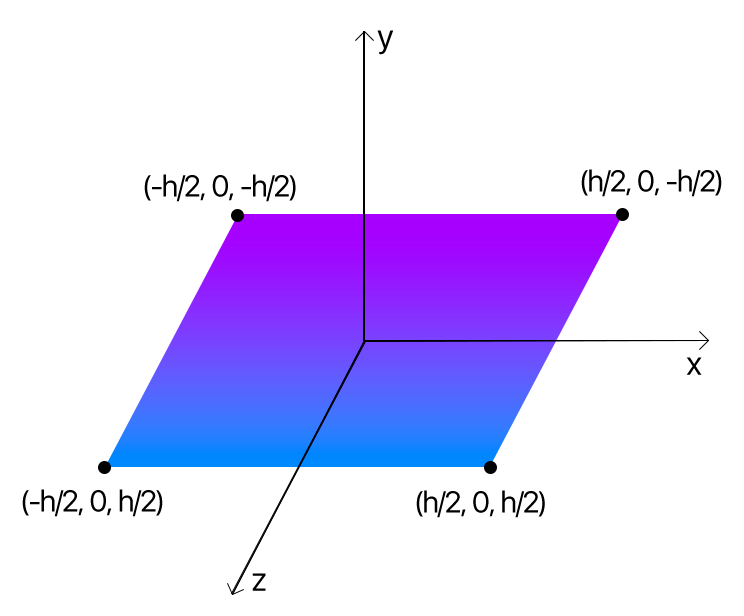
\includegraphics[width=\textwidth]{images/esquema_plano.png}
        \caption{coord dos pontos}
    \end{minipage}\hfill
    \begin{minipage}{0.33\textwidth}
        \centering
        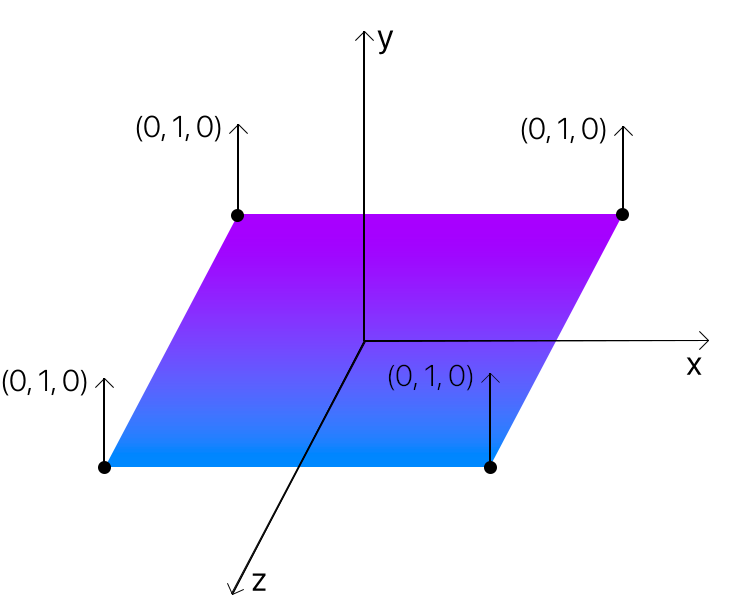
\includegraphics[width=\textwidth]{images/esquema_plano_normais.png}
        \caption{coord das normais}
    \end{minipage}\hfill
    \begin{minipage}{0.33\textwidth}
        \centering
        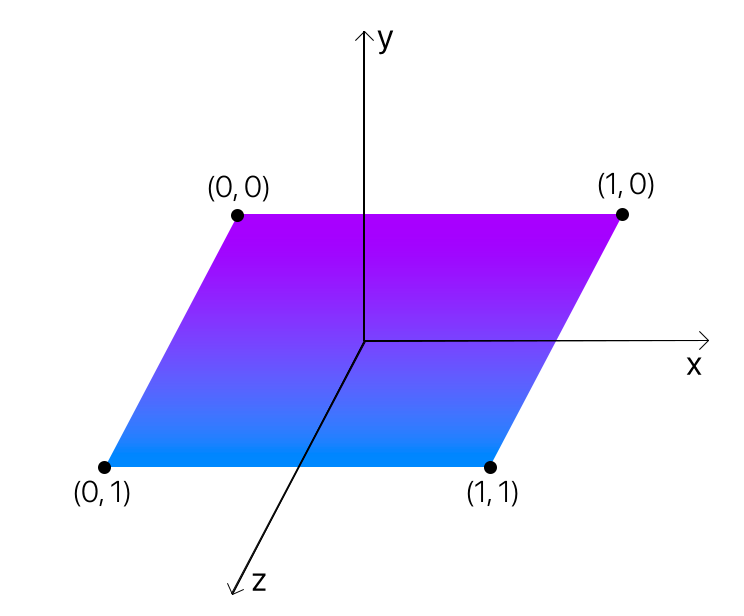
\includegraphics[width=\textwidth]{images/esquema_plano_textura.png}
        \caption{coord das texturas}
    \end{minipage}\hfill
\end{figure}

\begin{figure}[H]
    \centering
    \begin{minipage}{0.49\textwidth}
        \centering
        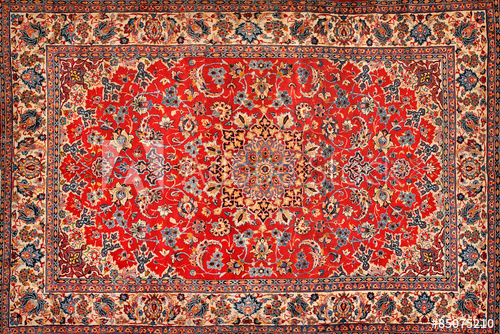
\includegraphics[width=\textwidth]{images/persian_carpet.jpg}
        \caption{exemplo de textura}
    \end{minipage}\hfill
    \begin{minipage}{0.5\textwidth}
        \centering
        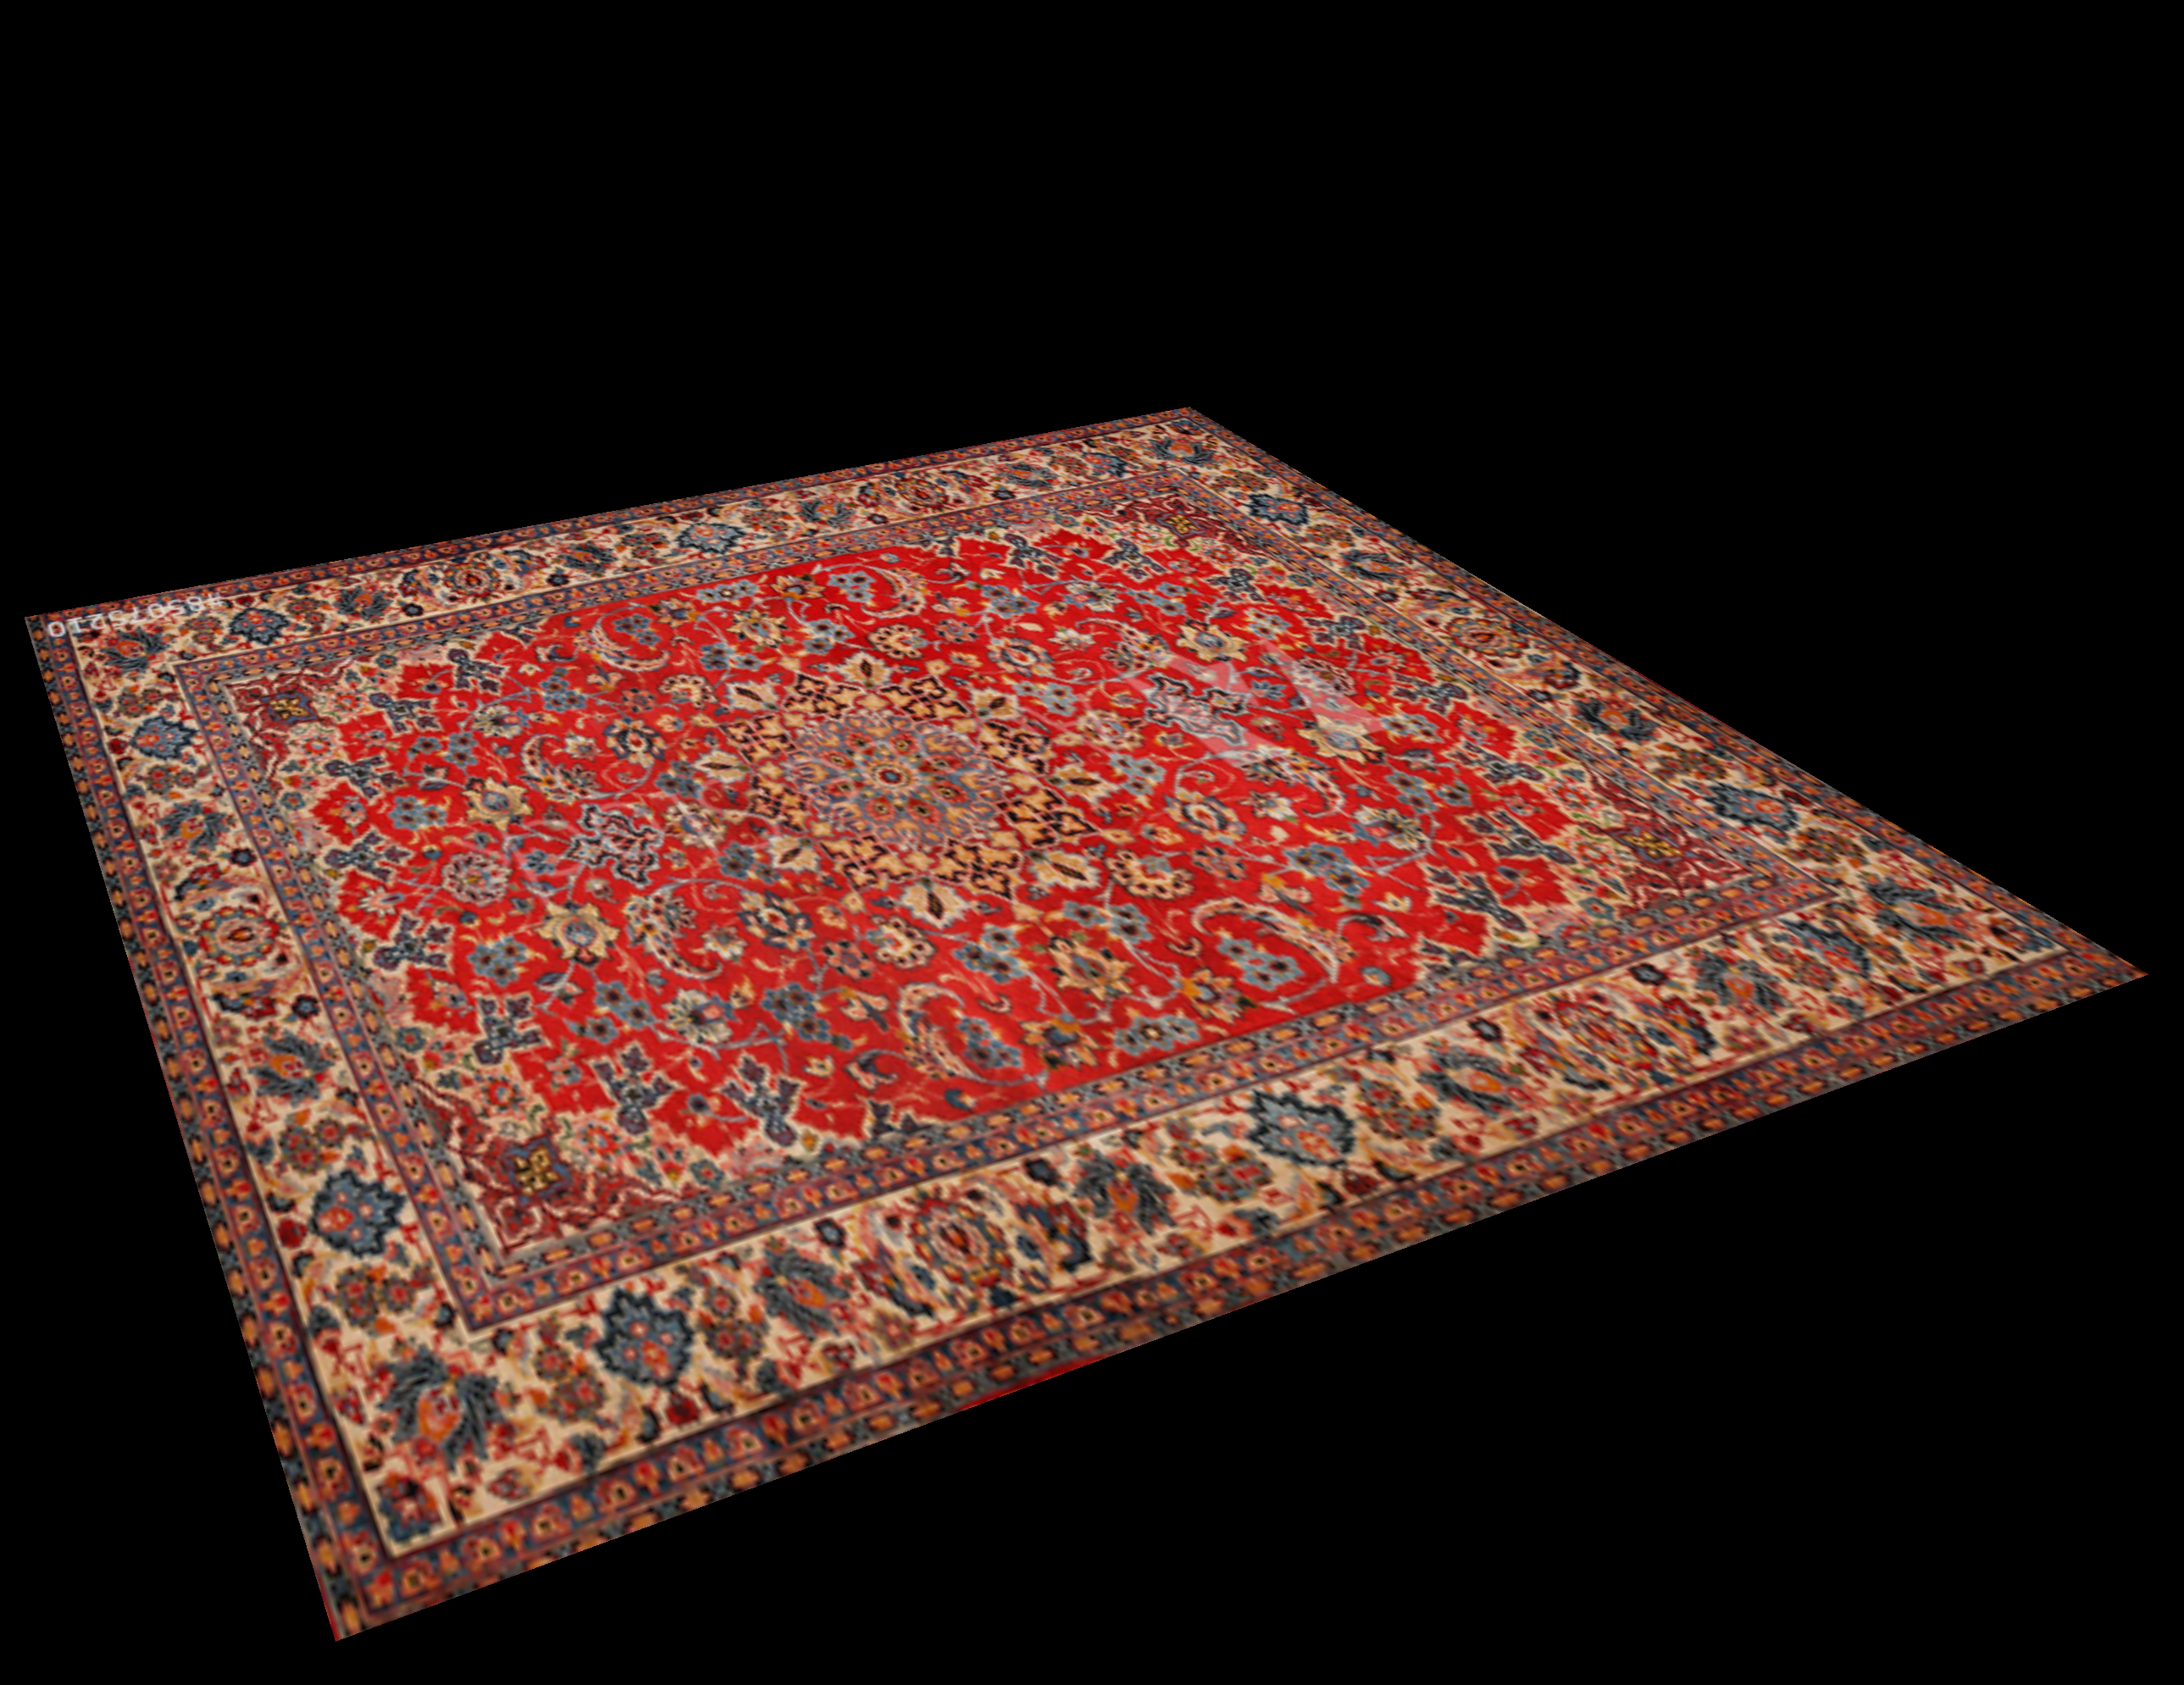
\includegraphics[width=\textwidth]{images/persian_carpet_rendered.png}
        \caption{resultado da textura}
    \end{minipage}\hfill
\end{figure}

\section{Esfera}
Para desenhar a esfera é necessário saber o seu raio (\textit{\_radius}), o
número de slices (\textit{\_slices}) e o número de stacks (\textit{\_stacks}).\\
Fazendo uso do sistema de coordenadas esférica basta calcular qual é o azimute e
qual é a inclinação de cada ponto (visto que o raio do pontos é igual ao raio da
esfera).\\
A normal de uma esfera num dado ponto é igual ao vetor normalizado do vetor que
vai do centro da esfera a um dado ponto. Para agilizar esta conta foi criado um
método na classe \textit{Point} que realiza estas contas
(\textit{normalized\_vector}).\\
Para facilitar estas contas são calculados dois valores, o ângulo entre cada
slice (\textit{a\_slice}) e o ângulo entre cada stack (\textit{a\_stack}).\\
As coordenadas de textura de uma esfera são semelhantes às de um mapa, sendo que
para calcular as coordenadas de textura de uma esfera basta ver em que slice e
em que stack está um dado ponto e dividir esses valores pelo número total de
slices e de stacks respetivamente.

\begin{lstlisting}
float curr_t_x = slice / _slices;
float curr_t_y = stack / _stacks;
float next_t_x = (slice + 1) / _slices;
float next_t_y = (stack + 1) / _stacks;
\end{lstlisting}

\begin{figure}[H]
    \centering
    \begin{minipage}{0.5\textwidth}
        \centering
        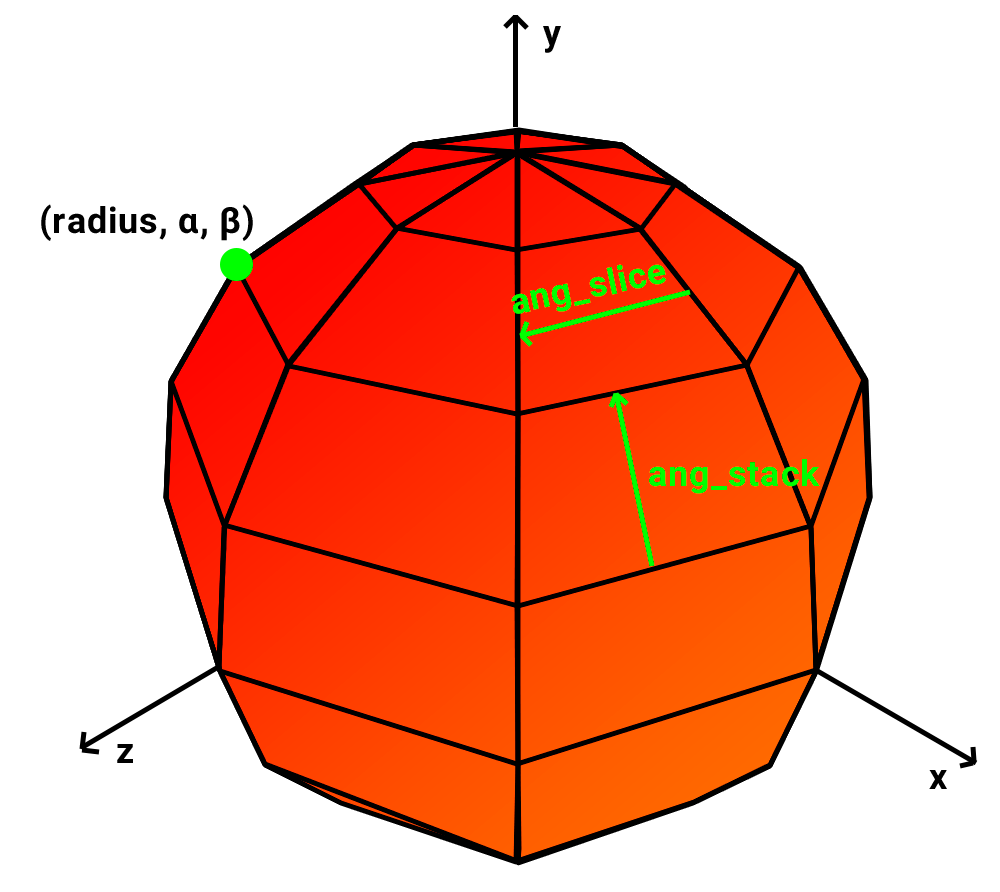
\includegraphics[width=\textwidth]{images/sphere_vetores.png}
        \caption{coord dos pontos}
    \end{minipage}\hfill
    \begin{minipage}{0.5\textwidth}
        \centering
        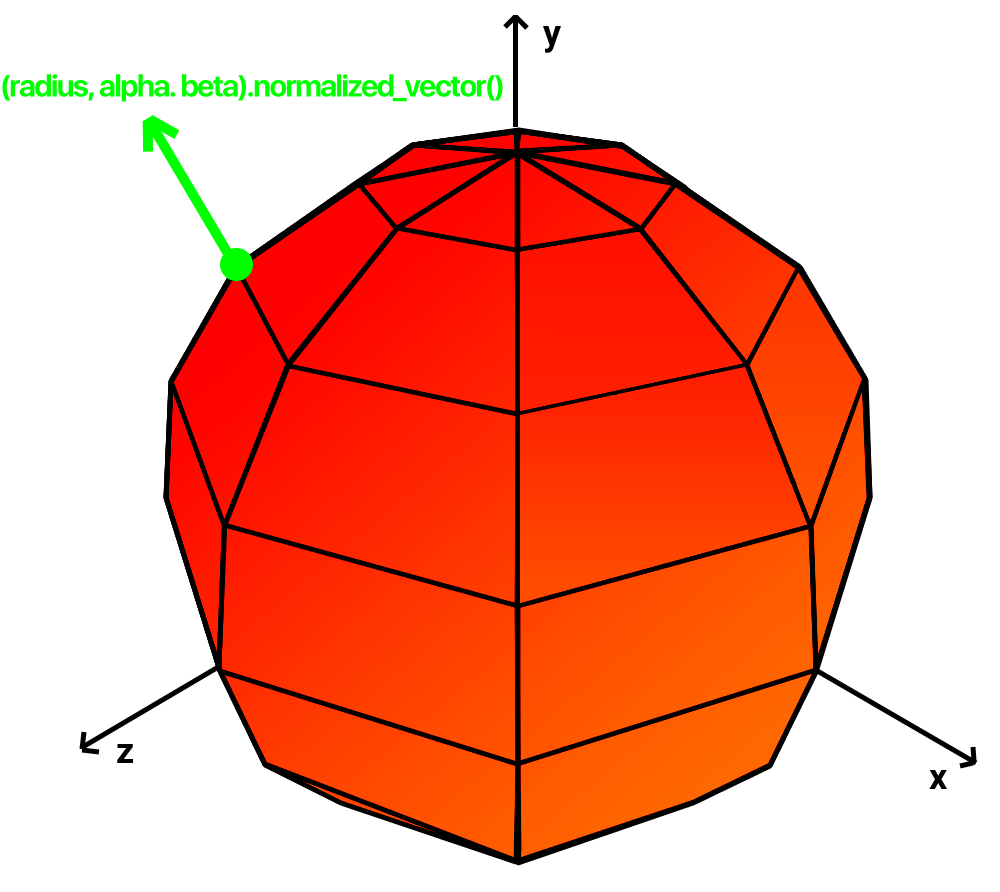
\includegraphics[width=\textwidth]{images/esfera_normal.png}
        \caption{coord das normais}
    \end{minipage}\hfill
\end{figure}
Para guardar os pontos calculados é criado um vetor de \textit{ModelPoint}
chamado \textit{coords}.

\begin{lstlisting}
    for (i32 slice = 0; slice < _slices; slice++) {
        for (i32 stack = 0; stack < _stacks; stack++) {
            auto p0 = PointSpherical(_radius, a_stack * stack, a_slice * slice);
            auto p1 = p0.add_inclination(a_stack);
            auto p2 = p0.add_azimuth(a_slice);
            auto p3 = p2.add_inclination(a_stack);

            auto v0 = p0.normalized_vector();
            auto v1 = p1.normalized_vector();
            auto v2 = p2.normalized_vector();
            auto v3 = p3.normalized_vector();

            if (stack != 0) {
                // 1st triangle
                coords.emplace_back(p2, v2, next_t_x, curr_t_y);
                coords.emplace_back(p0, v0, curr_t_x, curr_t_y);
                coords.emplace_back(p3, v3, next_t_x, next_t_y);
            }
            if (stack != _stacks - 1) {
                // 2nd triangle
                coords.emplace_back(p3, v3, next_t_x, next_t_y);
                coords.emplace_back(p0, v0, curr_t_x, curr_t_y);
                coords.emplace_back(p1, v1, curr_t_x, next_t_y);
            }
        }
    }
\end{lstlisting}


\begin{figure}[H]
    \centering
    \begin{minipage}{0.50\textwidth}
        \centering
        
\includegraphics[width=\textwidth]{images/basketball.png}
        \caption{exemplo de textura}
    \end{minipage}\hfill
    \begin{minipage}{0.49\textwidth}
        \centering
        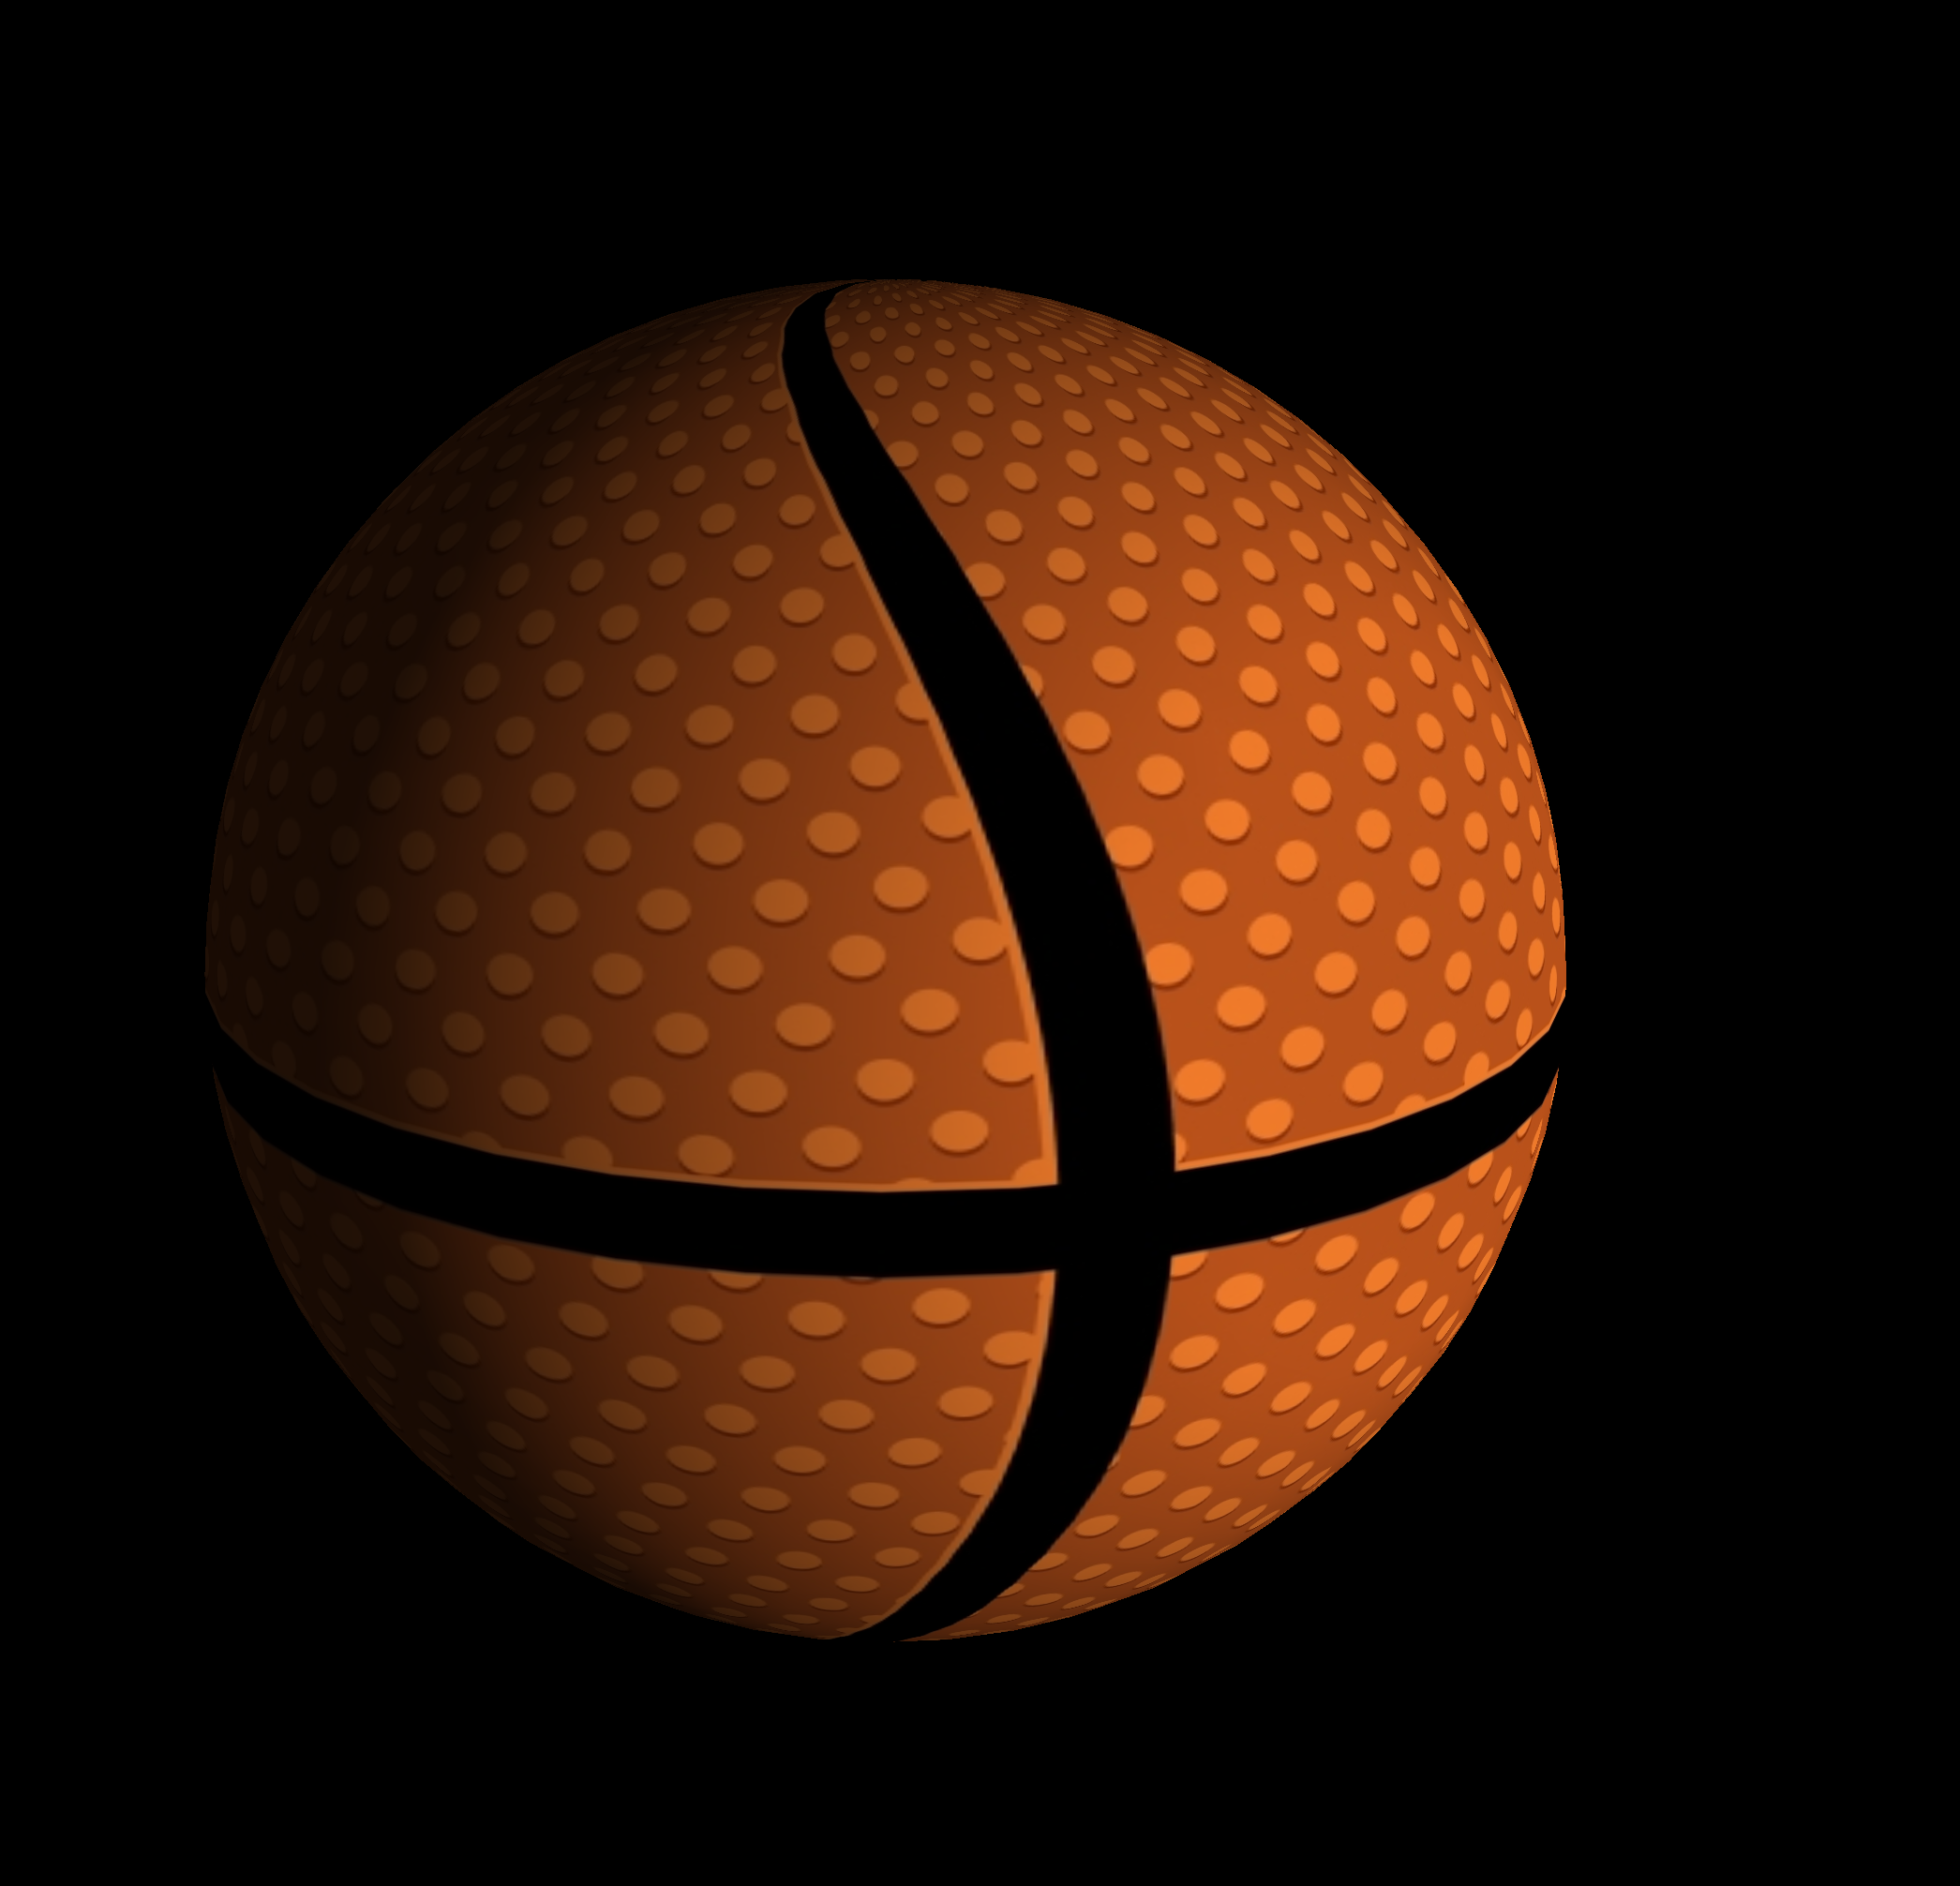
\includegraphics[width=\textwidth]{images/basket_rendered.png}
        \caption{resultado da textura}
    \end{minipage}\hfill
\end{figure}

\section{Torus}
Para desenhar uma Torus é preciso indicar o raio interior, o raio exterior, o
número de stacks(\textit{\_stacks} e o número de slices(\textit{\_slices}).\\
Para facilitar os cálculos estes valores são internamente convertidos para o
raio que vai do centro da torus ao centro do anel da torus (\textit{\_radius}) e
o raio do anel propriamente dito (\textit{\_ring\_radius}).

\begin{figure}[H]
    \centering 
    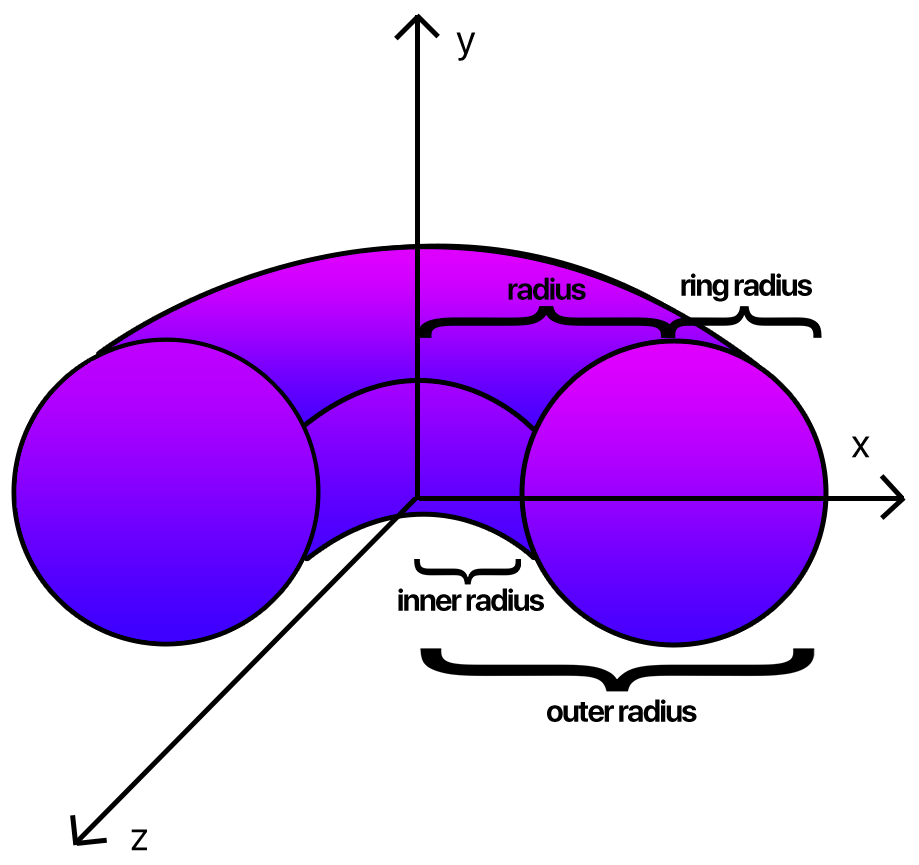
\includegraphics[width=0.5\textwidth]{images/torus_conversion.png}
    \caption{Esquema da conversão}
\end{figure}
Primeiro é definido o ângulo entre cada slice e cada stack com:

\begin{lstlisting}
float a_slice = 2.0f * M_PI / _slices;
float a_stack = 2.0f * M_PI / _stacks;
\end{lstlisting}
Para calcular as coordenadas de um ponto central da torus usamos coordenadas
esféricas. O raio é igual ao \textit{\_radius} e a inclinação é igual a $\pi$/2.
Logo, o único valor que varia é o azimute, que é igual a \textit{a\_slice} vezes
o índice da slice do ponto.\\
Com base nisto conseguimos calcular a coordenadas do ponto central de qualquer
\textit{slice}. Para calcular os triângulos do torus vai ser necessário ter o
ponto \textit{center} (que está na slice i) e o ponto \textit{n\_center} (que
está na slice i + 1).\\
Para calcular as coordenadas do ponto que está na superfície do torus precisamos
de calcular um vetor que vai do ponto calculado anteriormente até á
superfície. O raio deste vetor é fixo e é igual a \textit{\_ring\_radius} e o
azimute deste vetor é igual ao \textit{a\_stack} vezes a stack atual mais $\pi$
(para começar de baixo e assim corrigir as texturas). Logo, o único valor que
varia é a inclinação, que é igual a \textit{a\_stack} vezes o índice da stack
atual. Este vetor calculado se for normalizado com recurso ao método
\textit{normalize} é a normal do ponto.\\
\begin{figure}[H]
    \centering 
    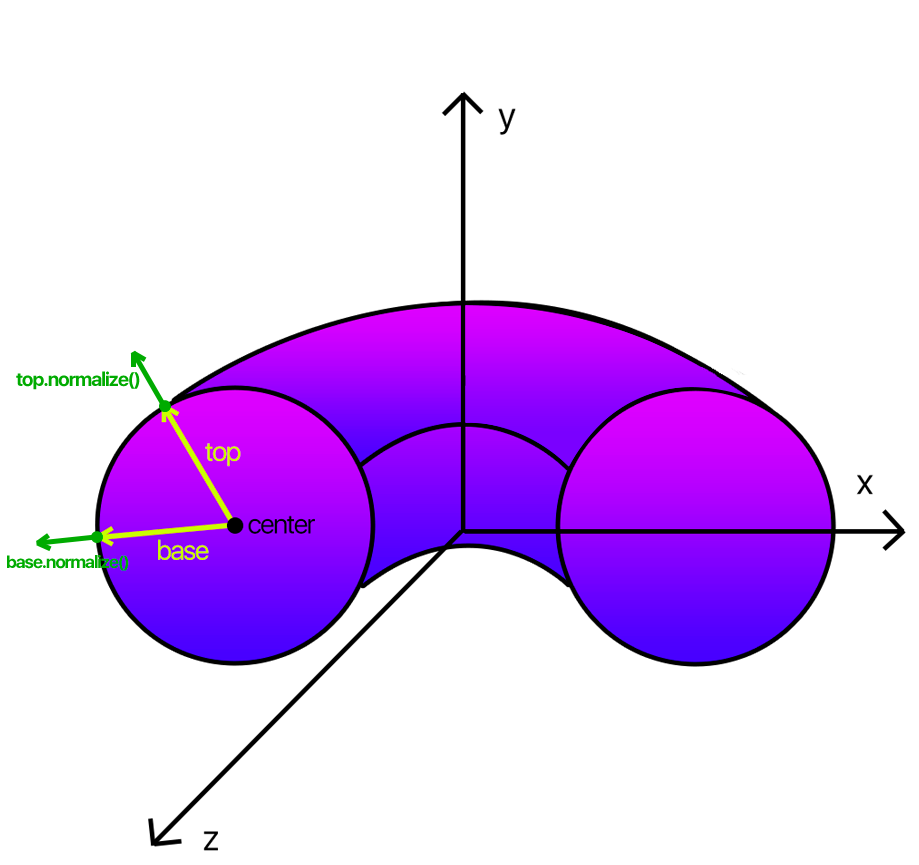
\includegraphics[width=0.5\textwidth]{images/torus_normal.png}
    \caption{Esquema da conversão}
\end{figure}
Somando para um dado ponto no centro do torus ao vetor correspondente obtemos o
ponto na superfície.\\
A maneira como calculamos as texturas do torus é semelhante à que usamos na
esfera  mas rodada 90º. Assim fica mais fácil criar e editar as texturas.\\
\begin{lstlisting}
float curr_t_x = stack / _stacks;
float curr_t_y = slice / _slices;
float next_t_x = (stack + 1) / _stacks;
float next_t_y = (slice + 1) / _slices;
\end{lstlisting}
Assim, para calcular os \textit{ModelPoint} e criar um vetor (\textit{coords})
com estes utilizamos o seguinte código.

\begin{lstlisting}
for (i32 slice = 0; slice < _slices; slice++) {
    for (i32 stack = 0; stack < _stacks; stack++) {
        // vetores do centro do torus ate a superficie
        float offset = a_stack * stack + M_PI;
        auto base = VectorSpherical(_ring_radius, offset, center.azimuth());
        auto n_base = base.add_azimuth(a_slice);
        auto top = base.add_inclination(a_stack);
        auto n_top = n_base.add_inclination(a_stack);

        // pontos na superficie
        auto p0 = center + base;
        auto p1 = center + top;
        auto p2 = n_center + n_base;
        auto p3 = n_center + n_top;

        // 1st triangle
        coords.emplace_back(p1, top.normalize(), top_t_x, curr_t_y);
        coords.emplace_back(p2, n_base.normalize(), base_t_x, next_t_y);
        coords.emplace_back(p0, base.normalize(), base_t_x, curr_t_y);

        // 2nd triangle
        coords.emplace_back(p1, top.normalize(), top_t_x, curr_t_y);
        coords.emplace_back(p3, n_top.normalize(), top_t_x, next_t_y);
        coords.emplace_back(p2, n_base.normalize(), base_t_x, next_t_y);
    }
}
\end{lstlisting}


\begin{figure}[H]
    \centering
    \begin{minipage}{0.40\textwidth}
        \centering
        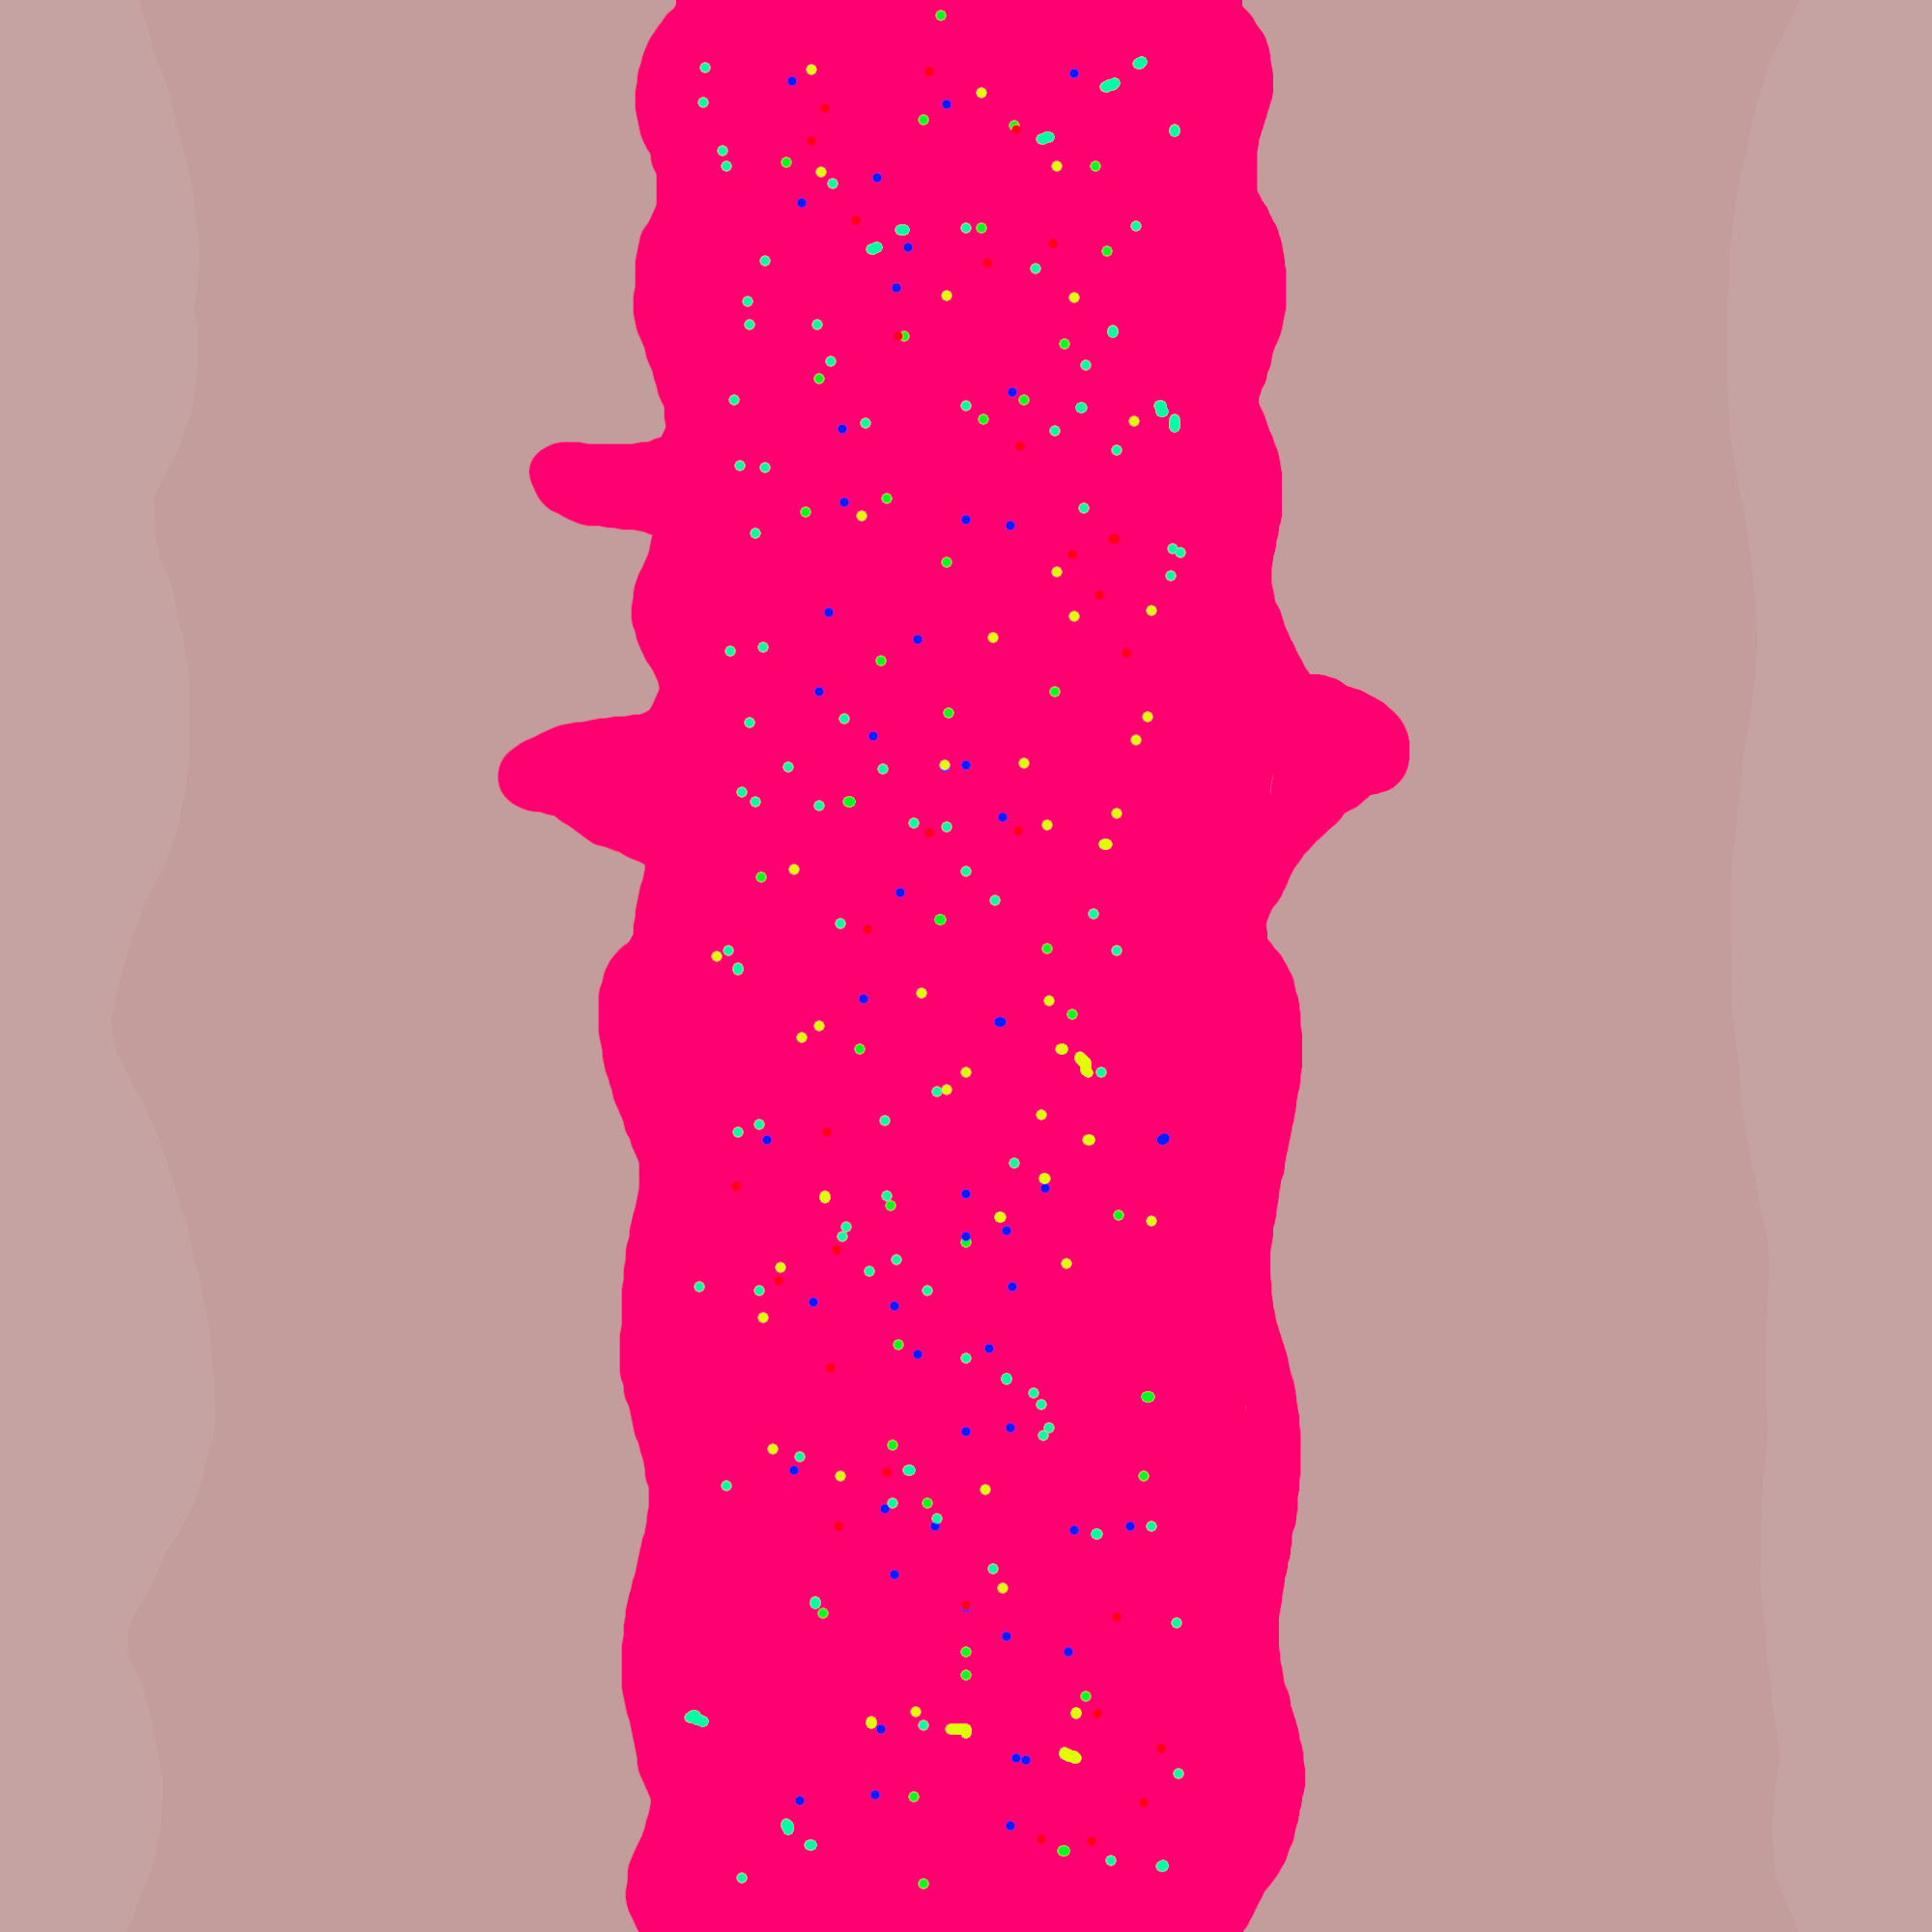
\includegraphics[width=\textwidth]{images/donut.jpg}
        \caption{exemplo de textura}
    \end{minipage}\hfill
    \begin{minipage}{0.59\textwidth}
        \centering
        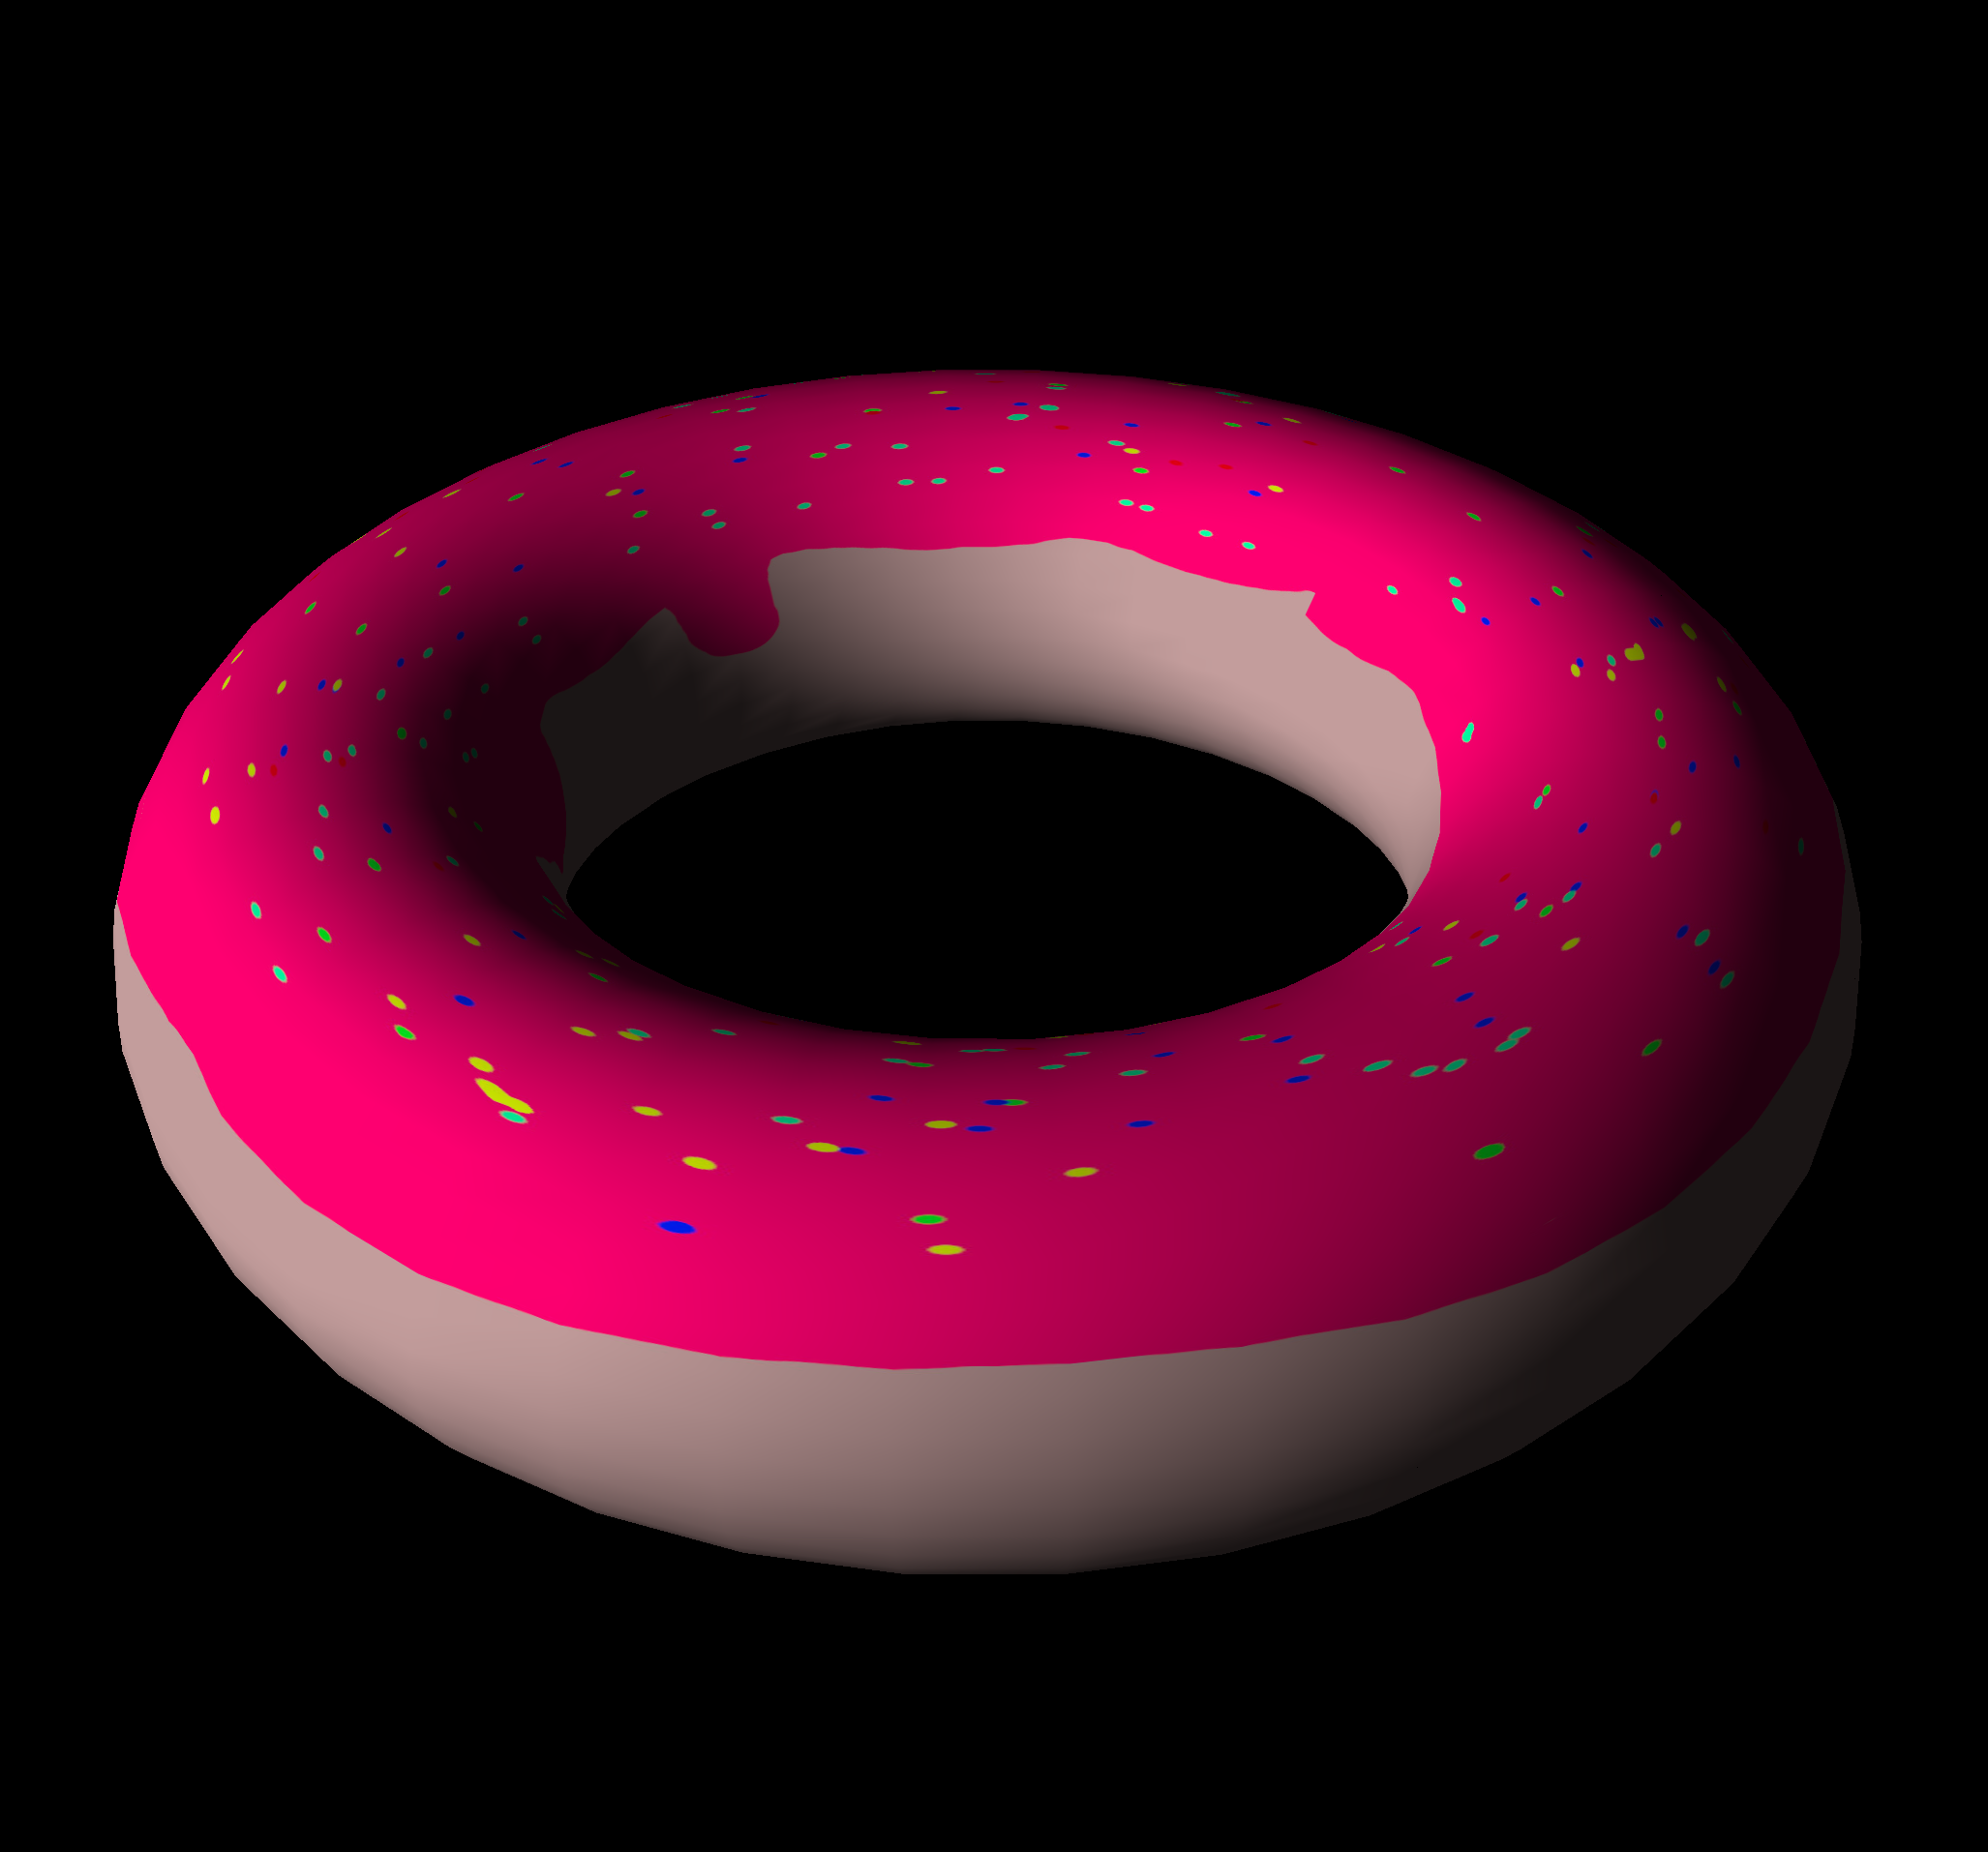
\includegraphics[width=\textwidth]{images/donut_rendered.png}
        \caption{resultado da textura}
    \end{minipage}\hfill
\end{figure}

\section{Cilindro}
Para desenhar um cilindro é necessário indicar o raio (\textit{\_radius}), a
altura (\textit{\_height}), o número de slices (\textit{\_slices}) e o número de
stacks (\textit{\_stacks}).\\
Com esta informação é calculado um vetor que vai da base do cilindro ao topo do
cilindro (\textit{top}). Dividindo este vetor pelo número de stacks obtemos um
vetor com o tamanho de cada uma das stacks. Em seguida dividimos 360º pelo
número total de slices (\textit{a\_slice}).\\
Assim, para um ponto da aresta da base numa dada slice é dado por
\textit{(radius, $\pi$/2, a\_slice * slice)}. Somando a este ponto o número da
slice do ponto vezes o vetor \textit{step} podemos calcular qualquer ponto na
face lateral do cilindro.
\begin{lstlisting}
Vector top = Vector(0, _height, 0);
Vector step = top / _stacks;
float a_slice = 2 * M_PI / _slices;
\end{lstlisting}
Em seguida definimos um ponto com coordenadas (0, 0, 0) denominado de
\textit{central}. Este ponto é o centro da base do cilindro. Para obter o
ponto central do topo do cilindro basta somar o vetor \textit{top} ao ponto
\textit{central}.\\
Para calcular um ponto ao longo da aresta da base (\textit{base}) do cilindro
utilizamos coordenadas esféricas. O raio da coordenada é igual ao raio do
cilindro e a inclinação é igual $\pi$/2 logo o único fator que varia é o
azimute. Para calcular este valor basta multiplicar o ângulo entre cada slice
pelo índice da slice onde o ponto se encontra. Desta forma, para obter as
coordenadas do ponto no índice seguinte (\textit{n\_base}) basta somar o ângulo
entre cada slice ao azimute do ponto.\\
O vetor normal é sempre o mesmo para todos os pontos da base do
cilindro e tem coordenadas (0, -1, 0) (\textit{bottom\_normal}). De forma
análoga, as normais dos pontos do topo do cilindro têm coordenadas (0, 1, 0)
(\textit{top\_normal}).\\
\begin{figure}[H]
    \centering 
    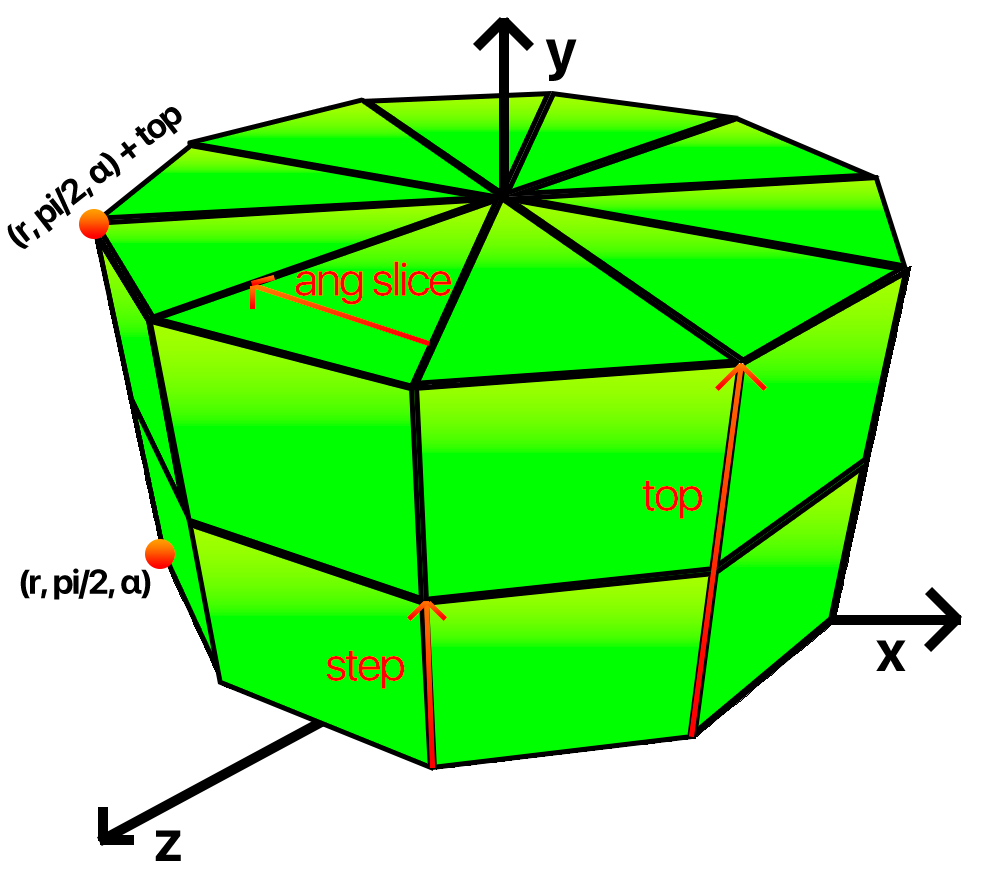
\includegraphics[width=0.5\textwidth]{images/cilindro_vetores.png}  
    \caption{Vetores e ângulos dos cilindros}
\end{figure}
Para calcular um ponto na lateral do cilindro primeiro utilizamos o que foi
definido no paragrafo anterior para criar um ponto na aresta da base do cilindro
na slice do ponto, depois somamos a este o vetor \textit{step} vezes o indice de
stack do ponto. O vetor normal a este ponto é o vetor que vai do ponto
\textit{central} ao ponto calculado na aresta da base do cilindro
(\textit{base\_v}).\\
\begin{figure}[H]
    \centering 
    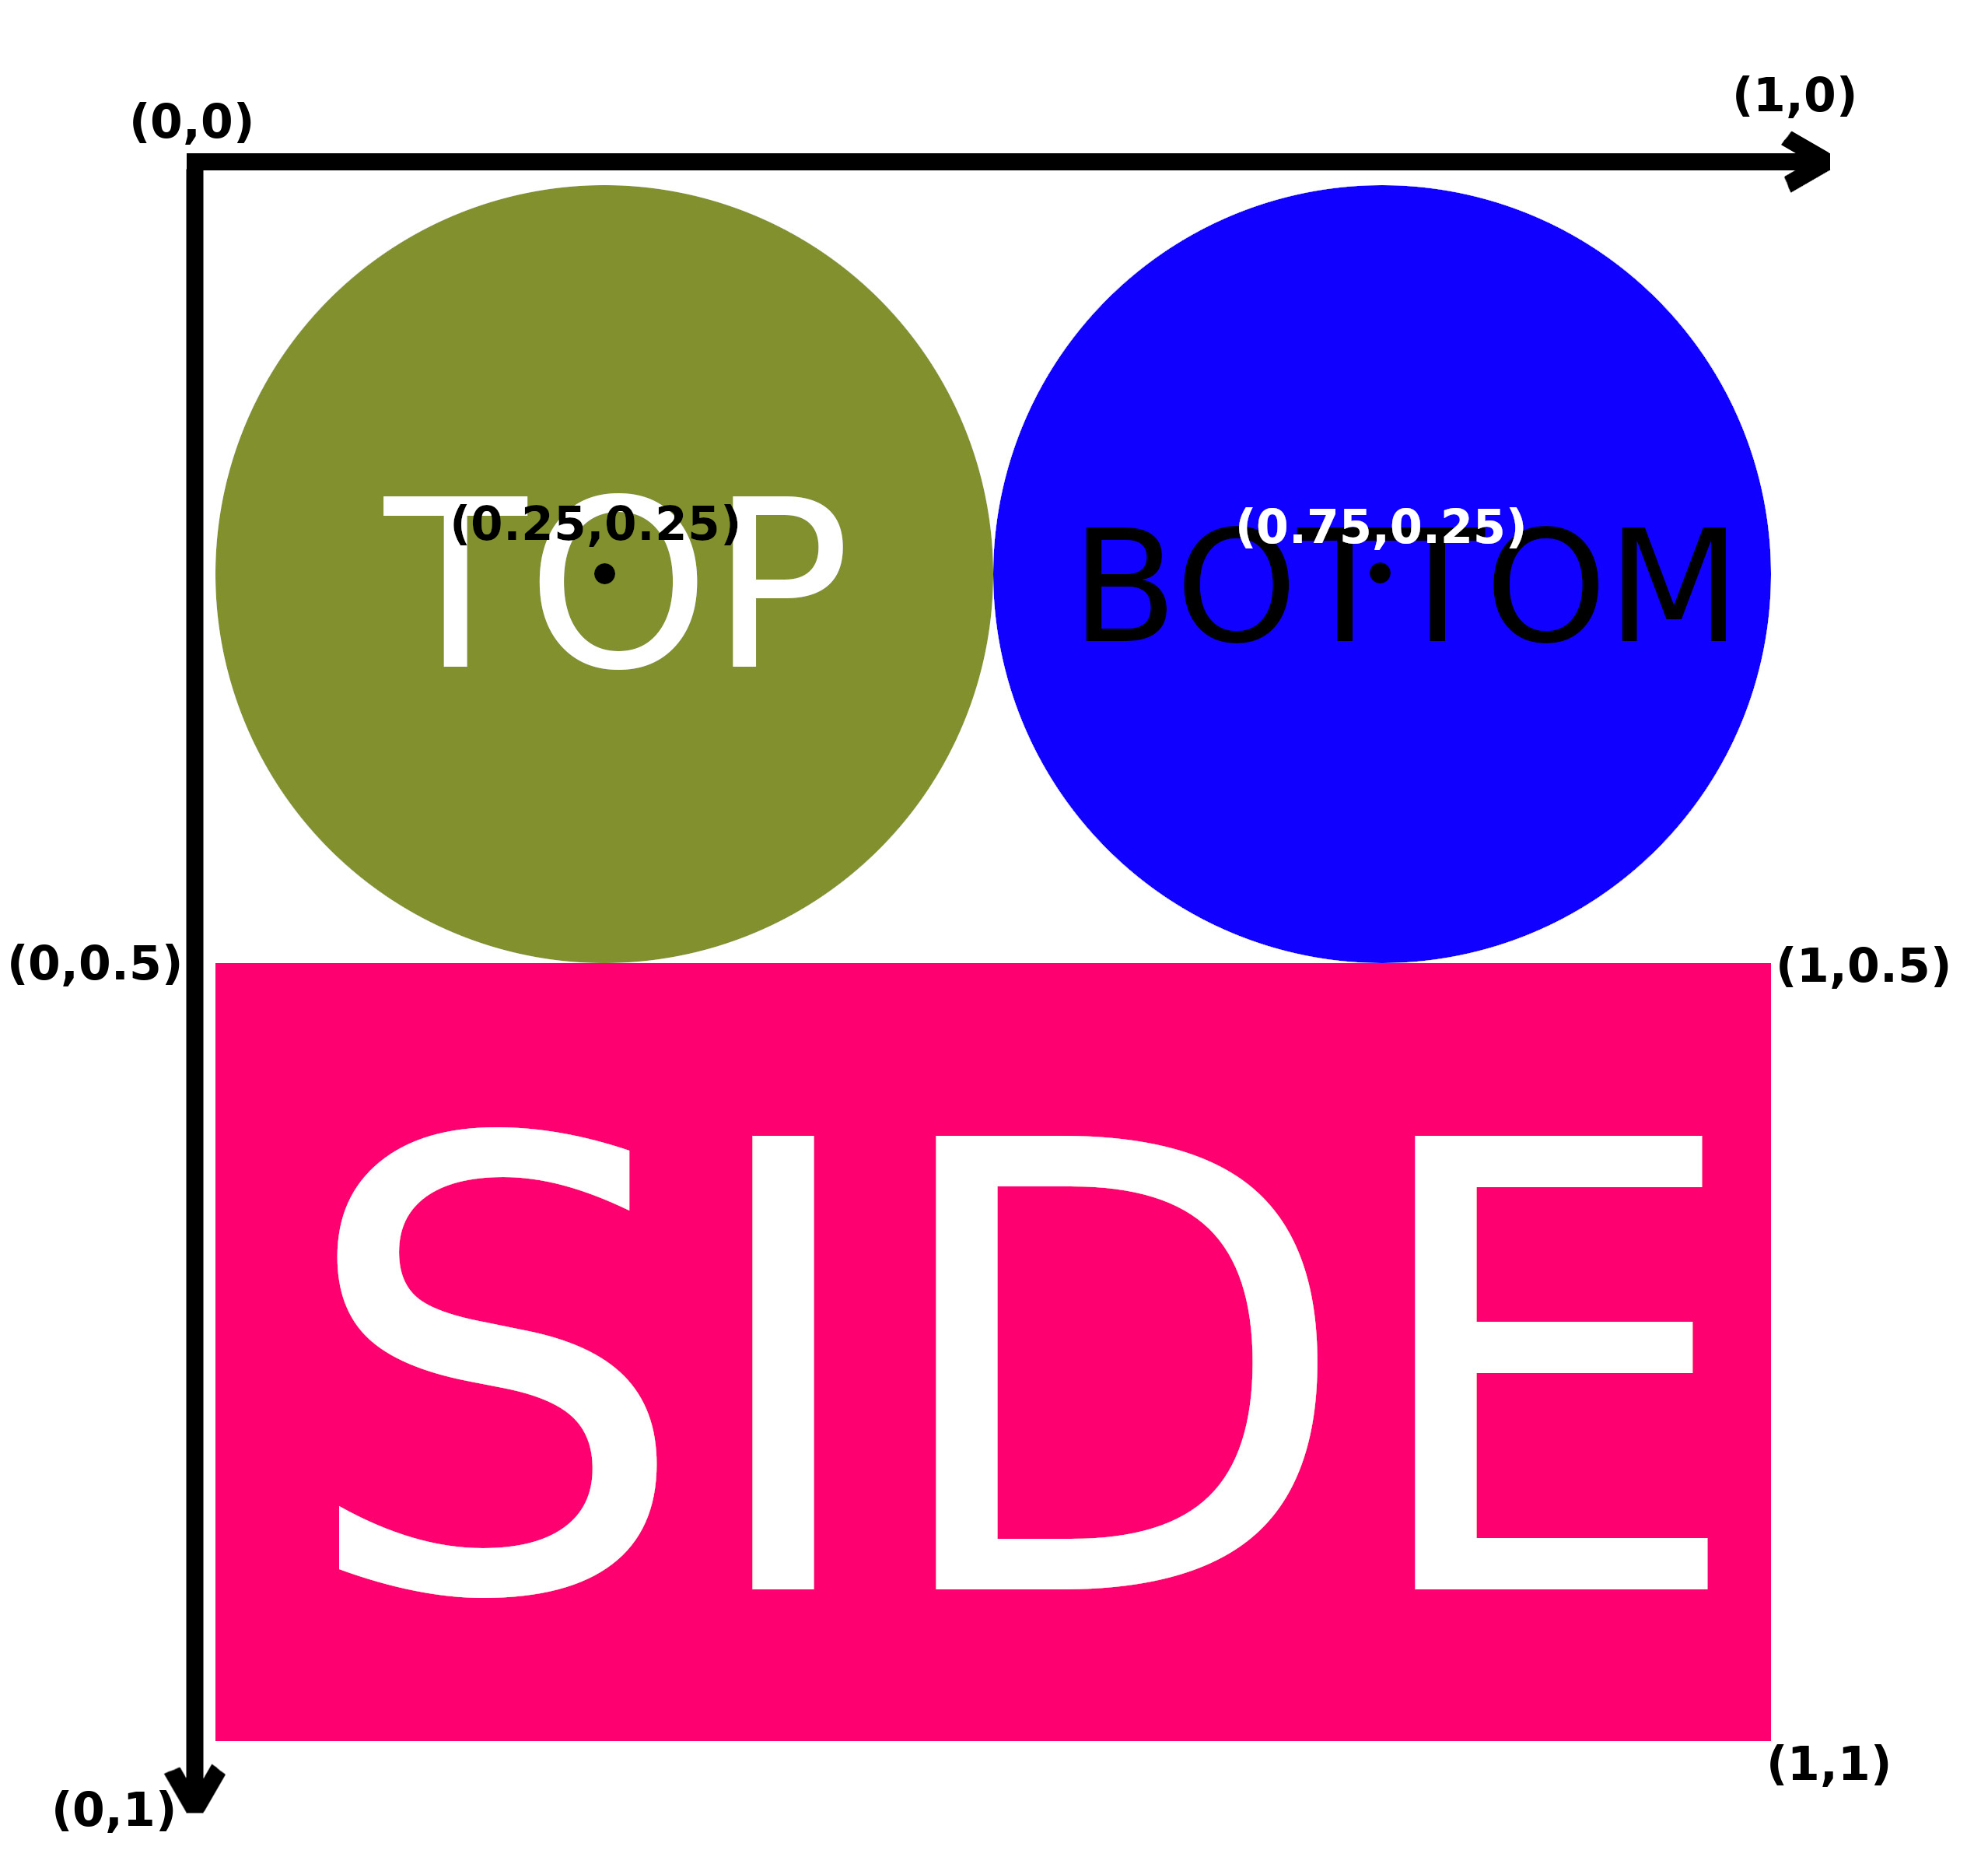
\includegraphics[width=0.5\textwidth]{images/cylinder_texture_scheme.png}  
    \caption{coordenadas de textura}
\end{figure}
Para facilitar o calculo das coordenadas de textura utilizamos os pontos 3D mas
apenas utilizando as coordenadas x e z.\\
Primeiro definimos um ponto no centro do círculo top, que tem coordenadas (0.25,
0, 0.25), denominado de \textit{t\_center} e outro no centro do circulo, com
coordenadas (0.75, 0, 0.25), denominado de \textit{b\_center}. Estes pontos
correspondem às coordenadas de textura dos pontos que estão no centro do topo e
da base do cilindro, respetivamente.\\
Para calcular as coordenadas de textura para os pontos da aresta do topo do
cilindro (\textit{t\_coor}) somamos às coordenadas do centro da textura o vetor
\textit{base\_v} multiplicado por 0.25. Desta forma, o vetor passa a ter o
comprimento do raio do circulo na imagem. Para a base do cilindro, o cálculo é
exatamente igual mas o vetor é espelhado no eixo dos z de forma a compensar o
facto de ser desenhado ao contrário (\textit{b\_coor}).\\
Finalmente, para calcular as coordenadas de textura no eixo do y para um dado
ponto dividimos o índice da slice do ponto em questão pelo número total de
slices ( \textit{curr\_t\_x}) e o eixo dos x é calculado por calcular 1 menos o
índice atual da stack a dividir pelo número total de stacks vezes 0.5. Desta
forma compensamos o facto de a lateral do cilindro ocupar metade da altura da
textura.\\
Assim, juntando tudo o que foi calculado, criamos os pontos e adicionamos a um
\textit{vector} de \textit{ModelPoint} chamado \textit{coords}.
\begin{lstlisting}
for (i32 slice = 0; slice < _slices; slice++) {
    // bottom
    coords.emplace_back( n_base, bottom_normal, n_b_coor.x(), n_b_coor.z());
    coords.emplace_back(   base, bottom_normal,   b_coor.x(),   b_coor.z());
    coords.emplace_back(central, bottom_normal, b_center.x(), b_center.z());

    // top
    coords.emplace_back(central + top, top_normal, t_center.x(), t_center.z());
    coords.emplace_back(base    + top, top_normal,   t_coor.x(),   t_coor.z());
    coords.emplace_back(n_base  + top, top_normal, n_t_coor.x(), n_t_coor.z());

    // side
    for (i32 stack = 0; stack < _stacks; stack++) {
        // 1st triangle
        coords.emplace_back(pivot, base_v, curr_t_x, curr_t_y);
        coords.emplace_back(n_pivot + step, n_base_v, next_t_x, next_t_y);
        coords.emplace_back(pivot + step, base_v, curr_t_x, next_t_y);

        // 2nd triangle
        coords.emplace_back(pivot, base_v, curr_t_x, curr_t_y);
        coords.emplace_back(n_pivot, n_base_v, next_t_x, curr_t_y);
        coords.emplace_back(n_pivot + step, n_base_v, next_t_x, next_t_y);
    }
}
\end{lstlisting}

\begin{figure}[H]
    \centering
    \begin{minipage}{0.40\textwidth}
        \centering
        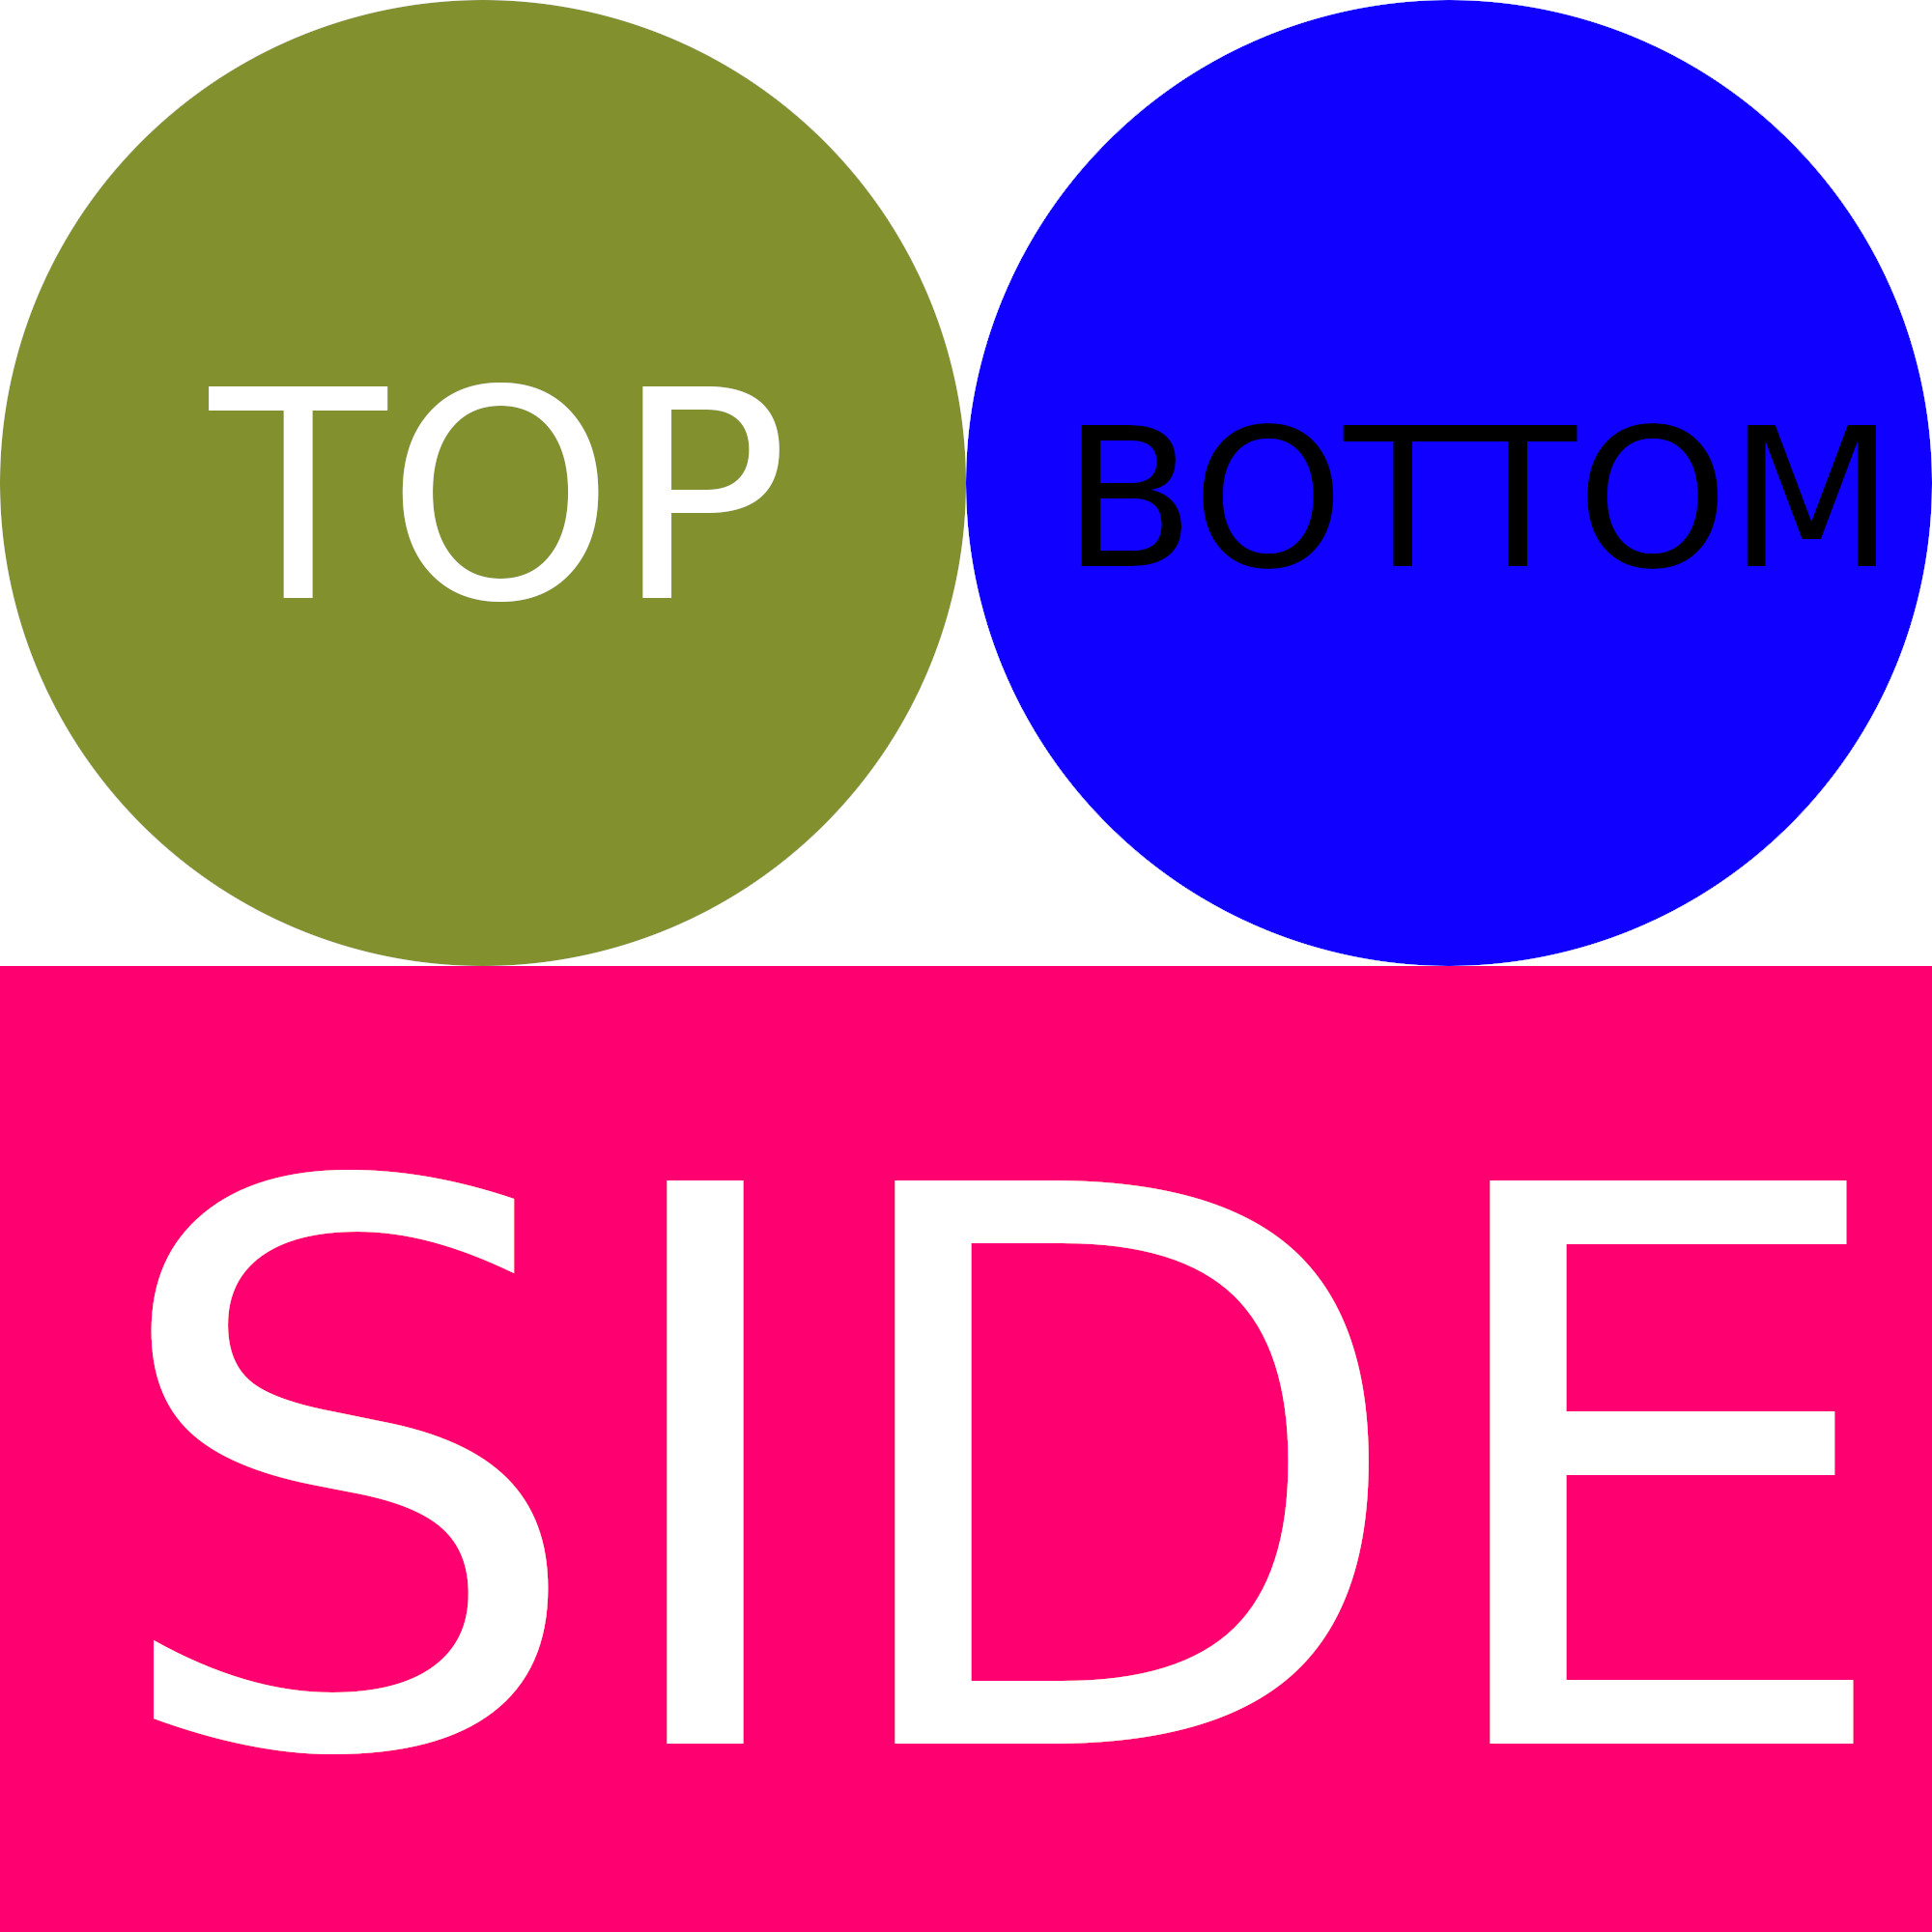
\includegraphics[width=\textwidth]{images/cylinder_texture.jpg}
        \caption{exemplo de textura}
    \end{minipage}\hfill
    \begin{minipage}{0.59\textwidth}
        \centering
        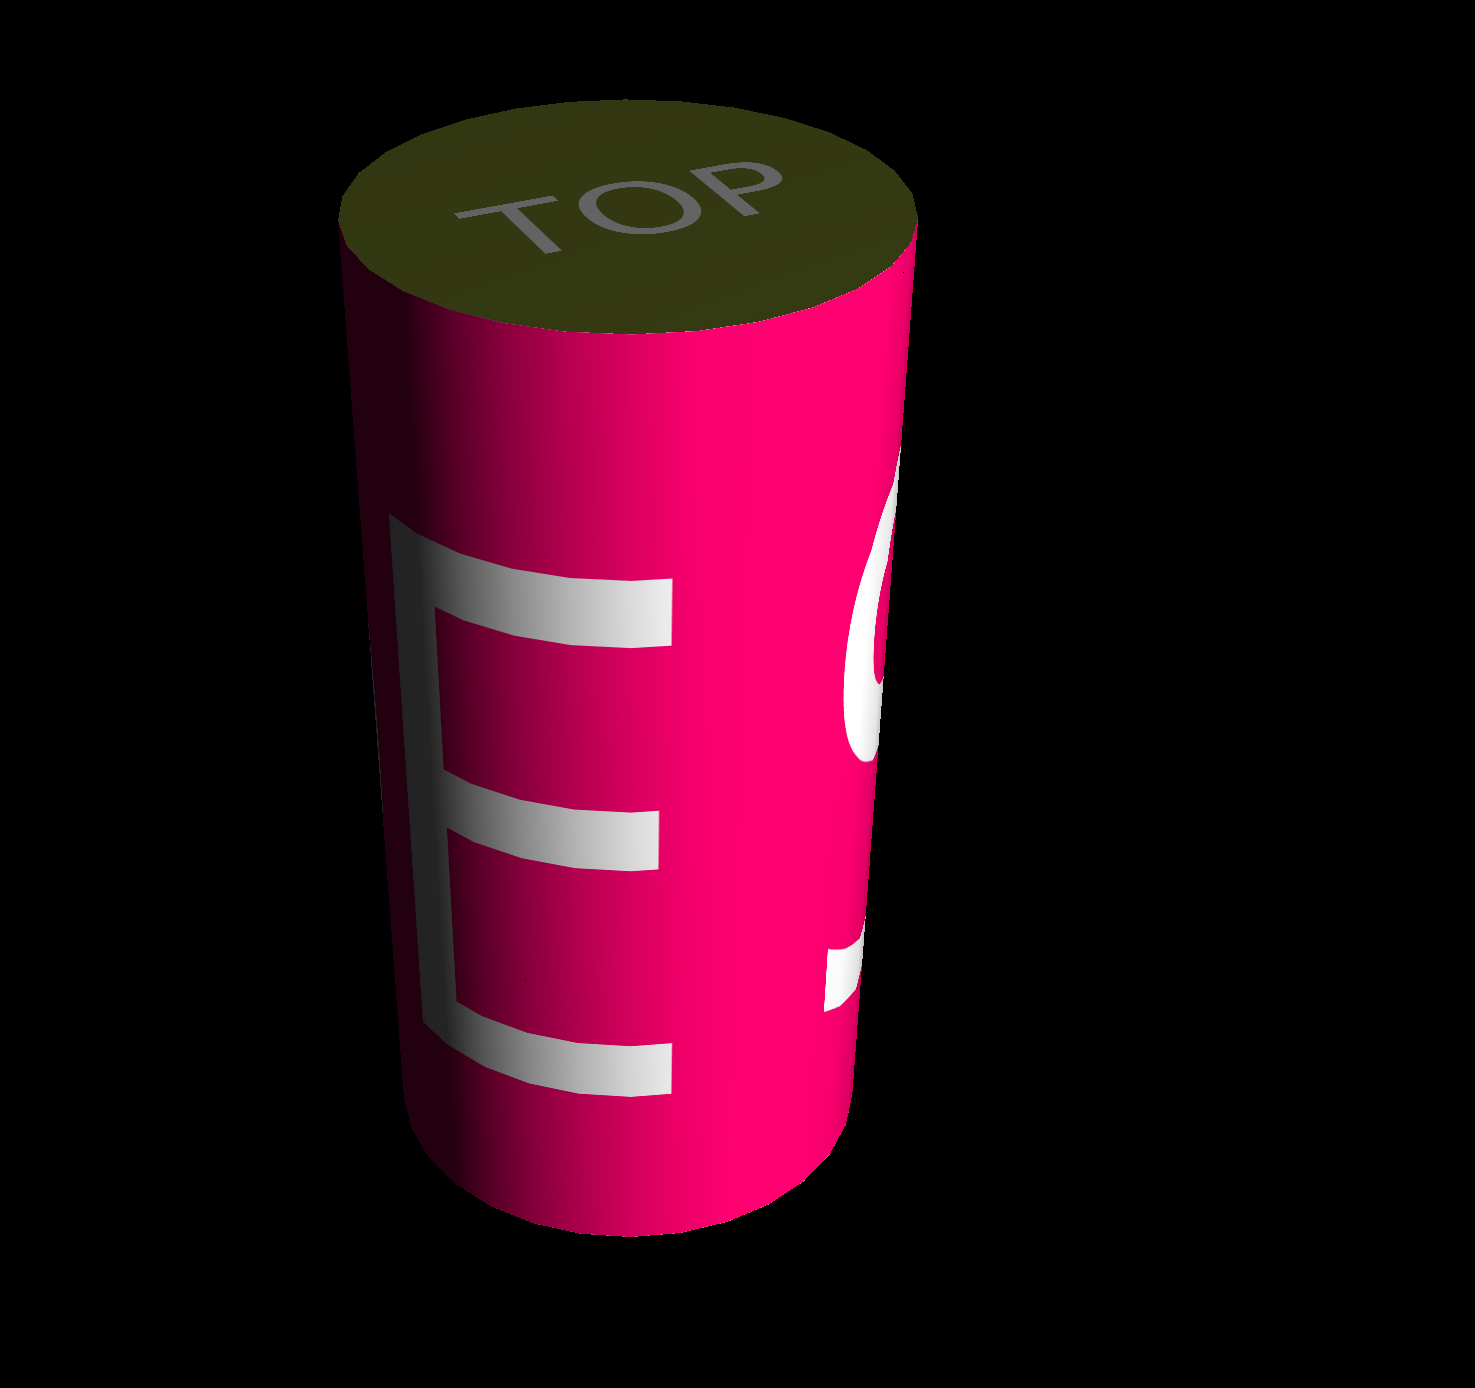
\includegraphics[width=\textwidth]{images/cylinder_rendered.png}
        \caption{resultado da textura}
    \end{minipage}\hfill
\end{figure}

\section{Cone}
\begin{figure}[H]
    \centering
    \begin{minipage}{0.40\textwidth}
        \centering
        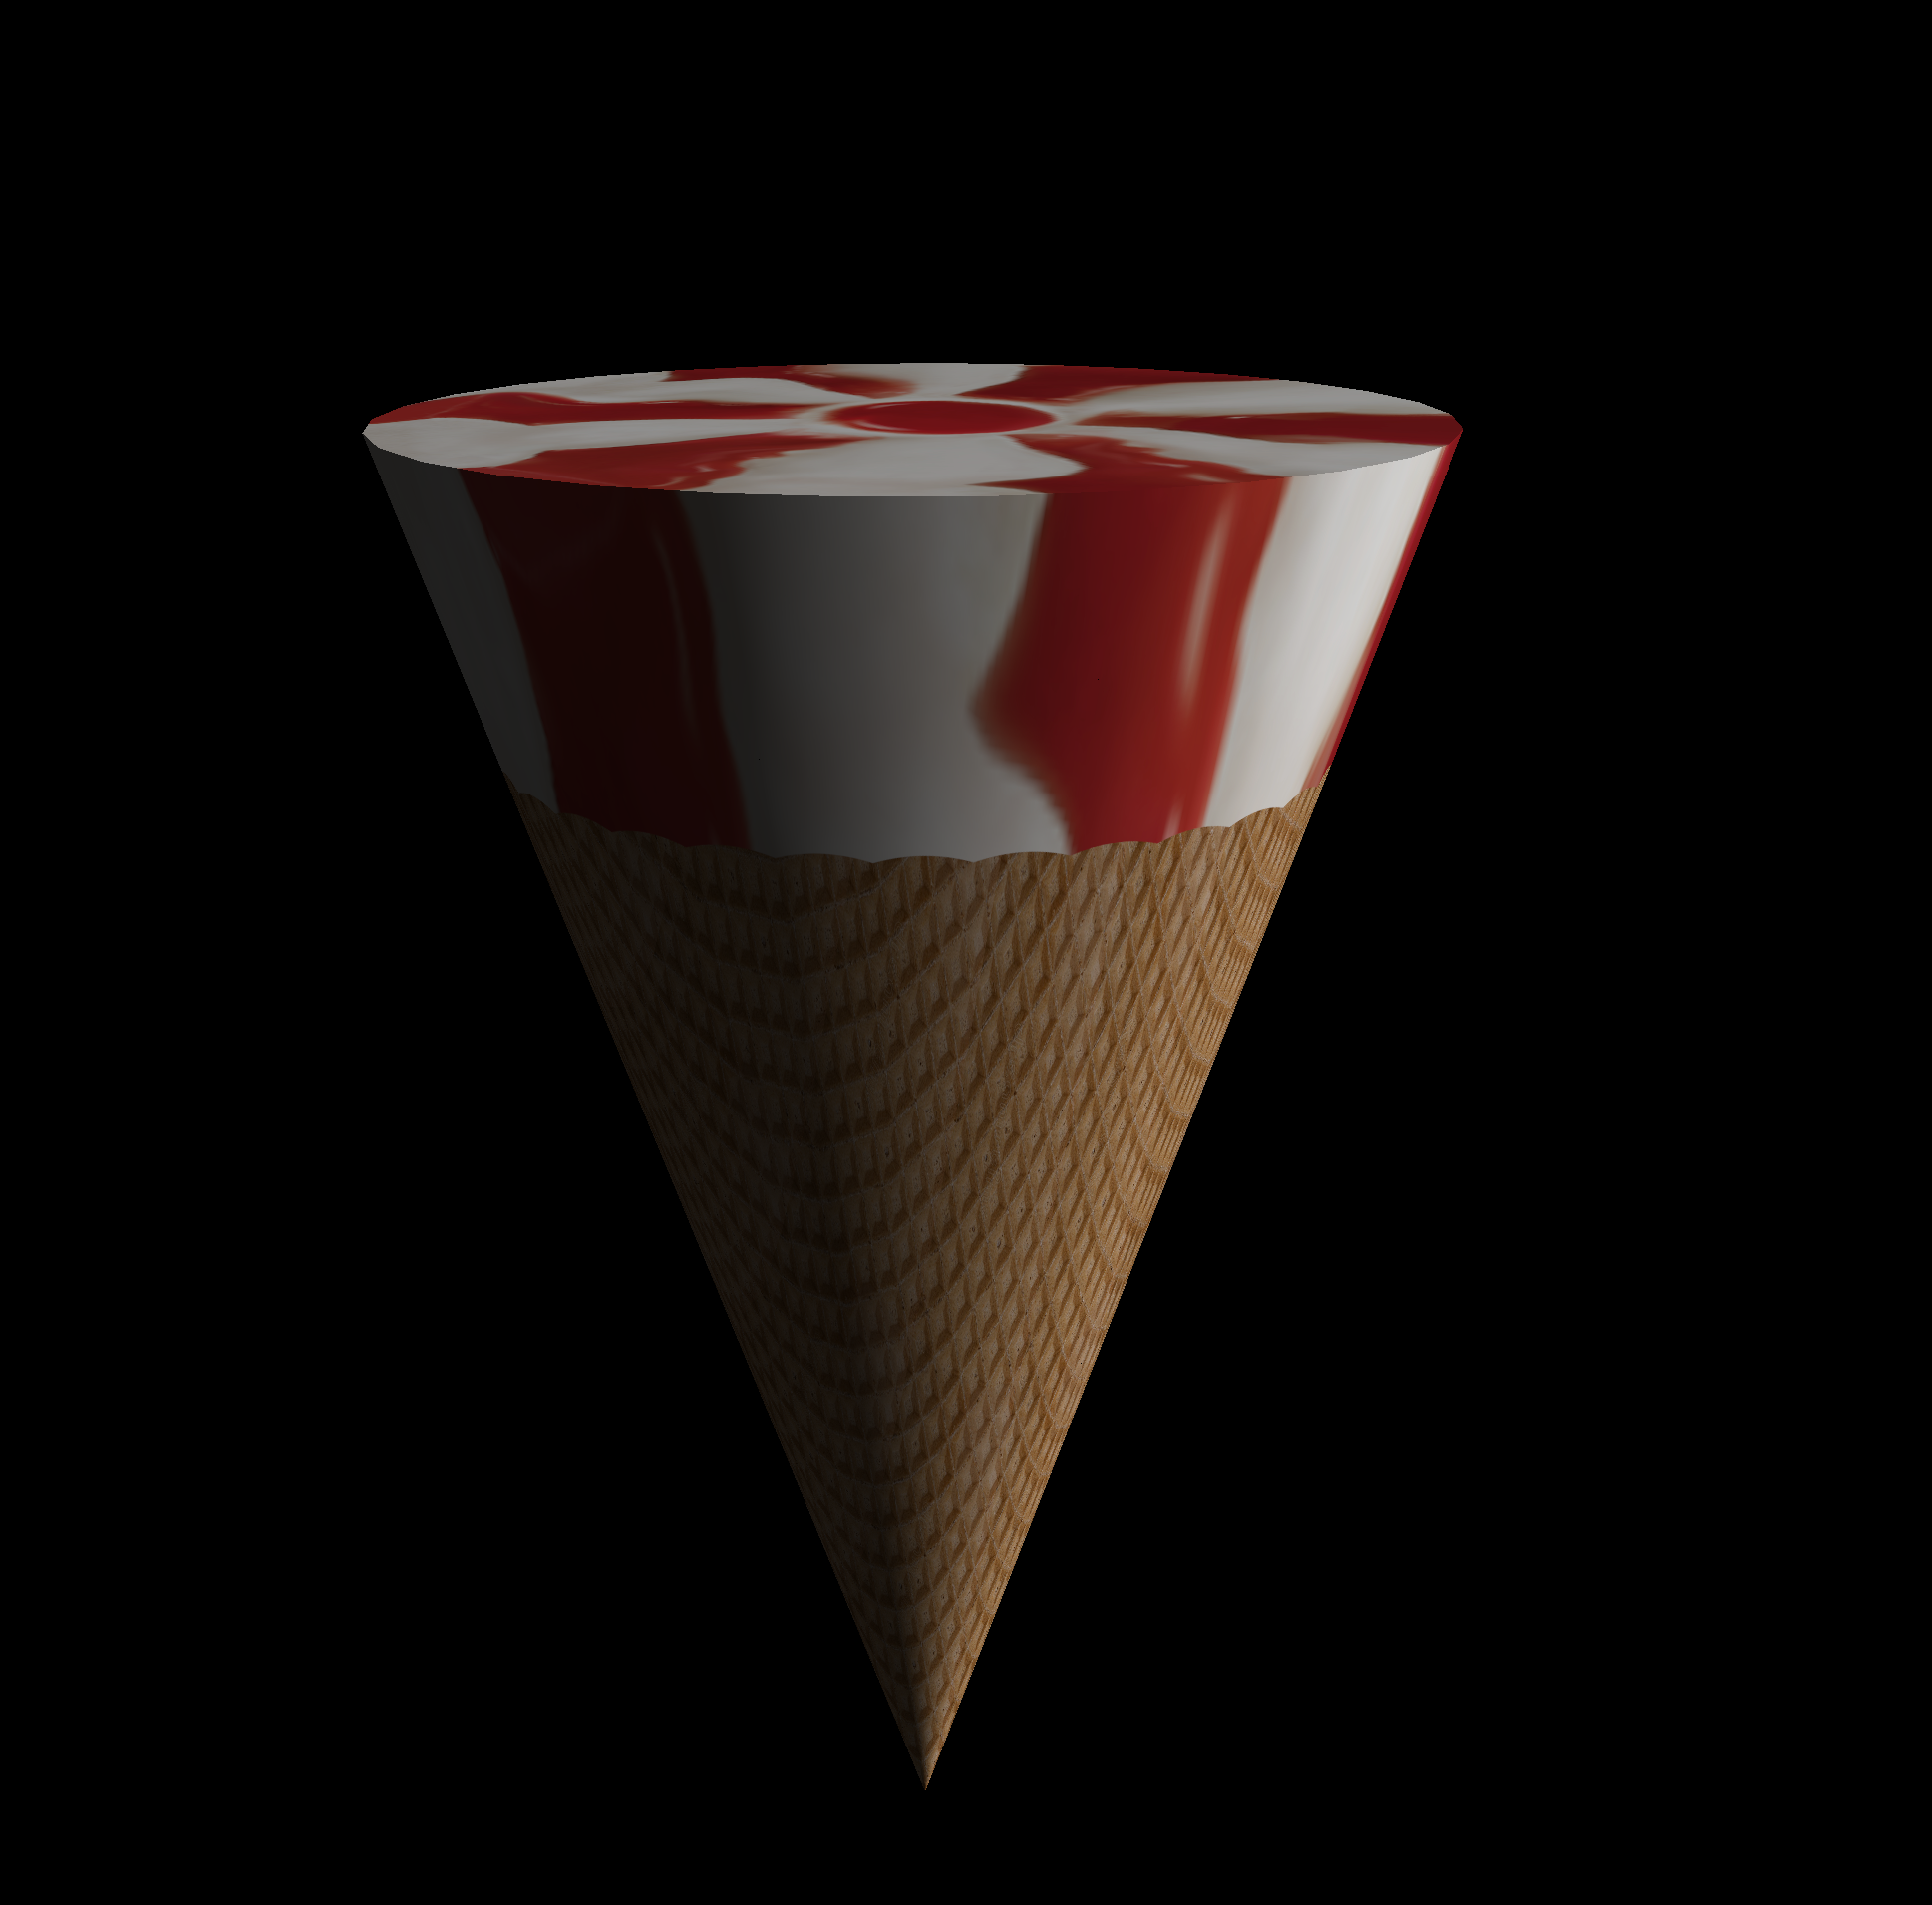
\includegraphics[width=\textwidth]{images/corneto.jpg}
        \caption{exemplo de textura}
    \end{minipage}\hfill
    \begin{minipage}{0.59\textwidth}
        \centering
        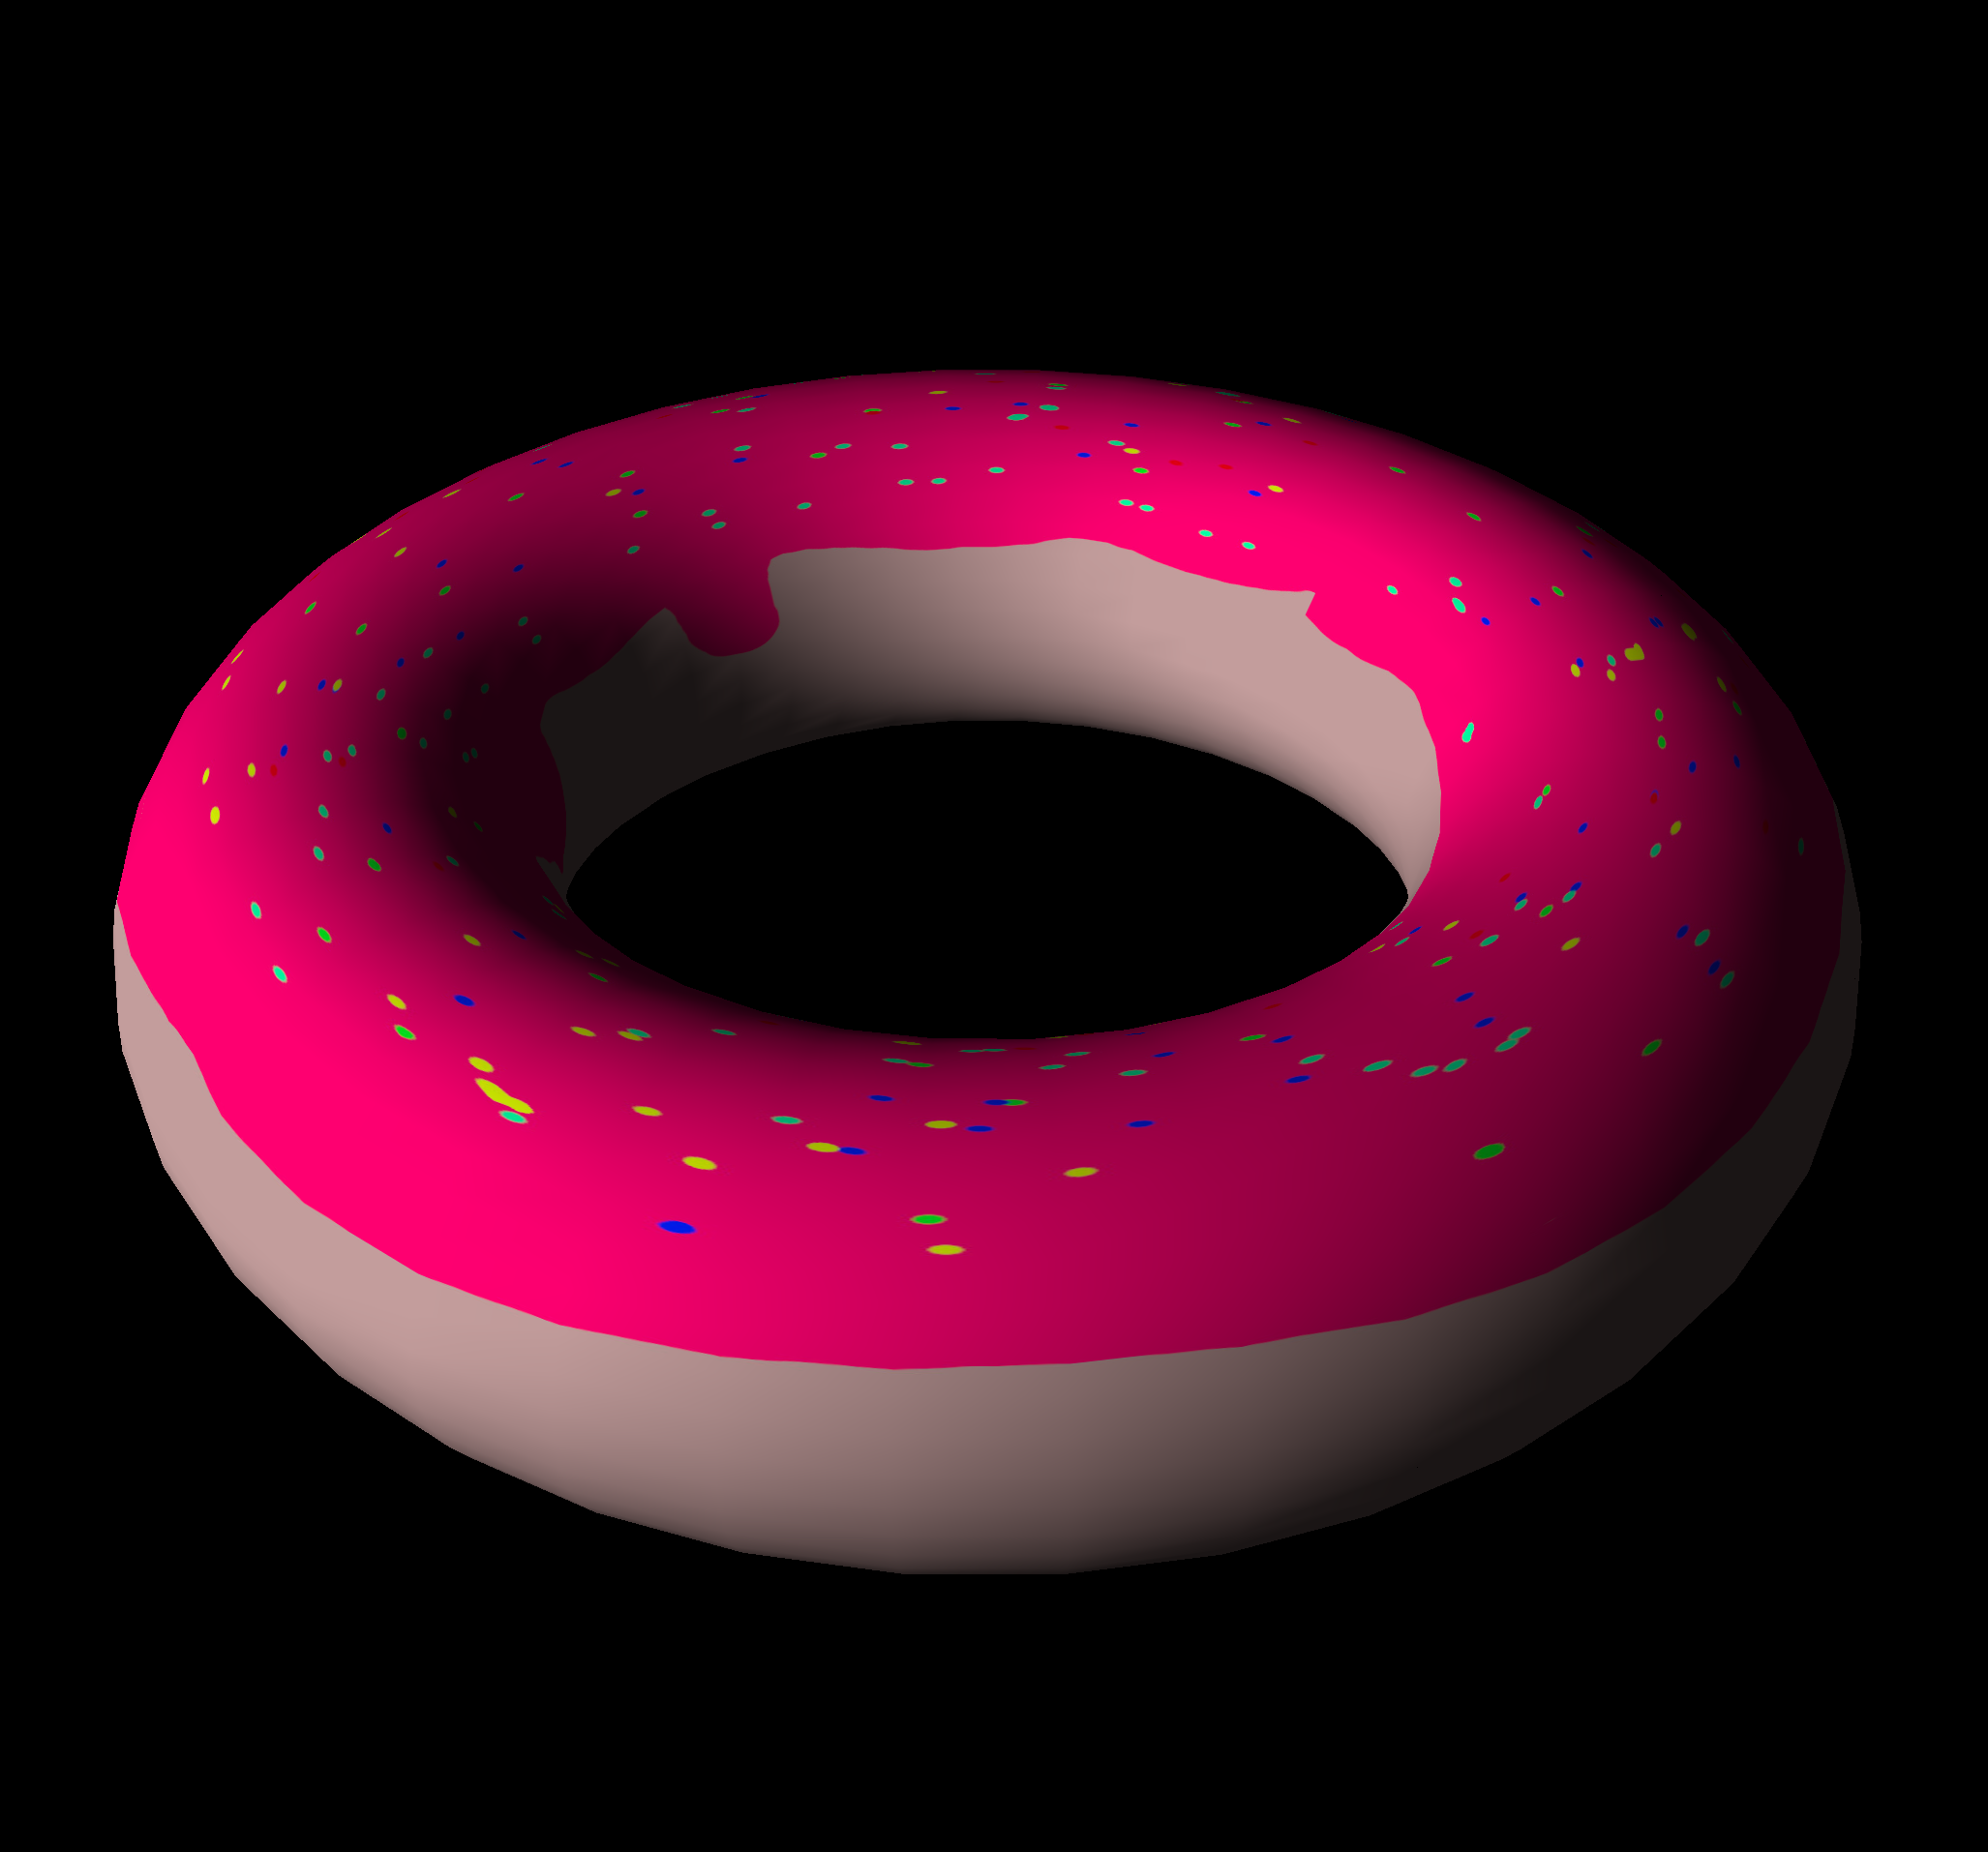
\includegraphics[width=\textwidth]{images/donut_rendered.png}
        \caption{resultado da textura}
    \end{minipage}\hfill
\end{figure}

\section{Caixa}
Para gerar uma caixa é necessário saber as 3 dimensões (\textit{\_x},
\textit{\_y} e \textit{\_z})  e o número de
divisões da caixa (\textit{\_slices}).\\
Primeiro calculamos 3 vetores distintos. Cada um alinhado com um dos eixos no
sentido positivo e com comprimento o tamanho de uma divisão da caixa.\\
Em seguida calculamos mais 3 vetores com bases nestes três que têm exatamente o
mesmo comprimento mas sentido inverso.\\
Em seguida criamos um conjunto de 6 pontos que indicam as coordenadas onde
começam cada textura.\\
Para calcular cada face foi criada uma função auxiliar que recebe o ponto no
espaço onde começa a face, as coordenadas da textura equivalentes a esse ponto e
2 vetores dos calculados anteriormente de forma a que estejam alinhados com a
aresta da face e que o seu \textit{cross product} seja normal à face.\\
Tal como já foi referido basta fazer o cross product dos dois vetores para obter
a normal de todos os pontos da face.\\
Para obter um ponto (n, m) na face da caixa basta multiplicar por n um dos
vetores e multiplicar por m o outro, e somar estes vetores ao ponto de origem da
face.\\
Da mesma forma, para calcular as coordenadas da textura de um ponto sabendo que
ele está na posição (n, m) utilizamos a fórmula para obter o \textit{offset}
relativamente ao ponto de origem passado como parâmetro. As multiplicações por 3 e
por 2 servem para compensar o facto de só se usar 1/6 da área da textura para
cada face.
\begin{lstlisting}
float xt = i / (_slices * 3);
float yt = j / (_slices * 2);
\end{lstlisting}

\begin{figure}[H]
    \centering
    \begin{minipage}{0.39\textwidth}
        \centering
        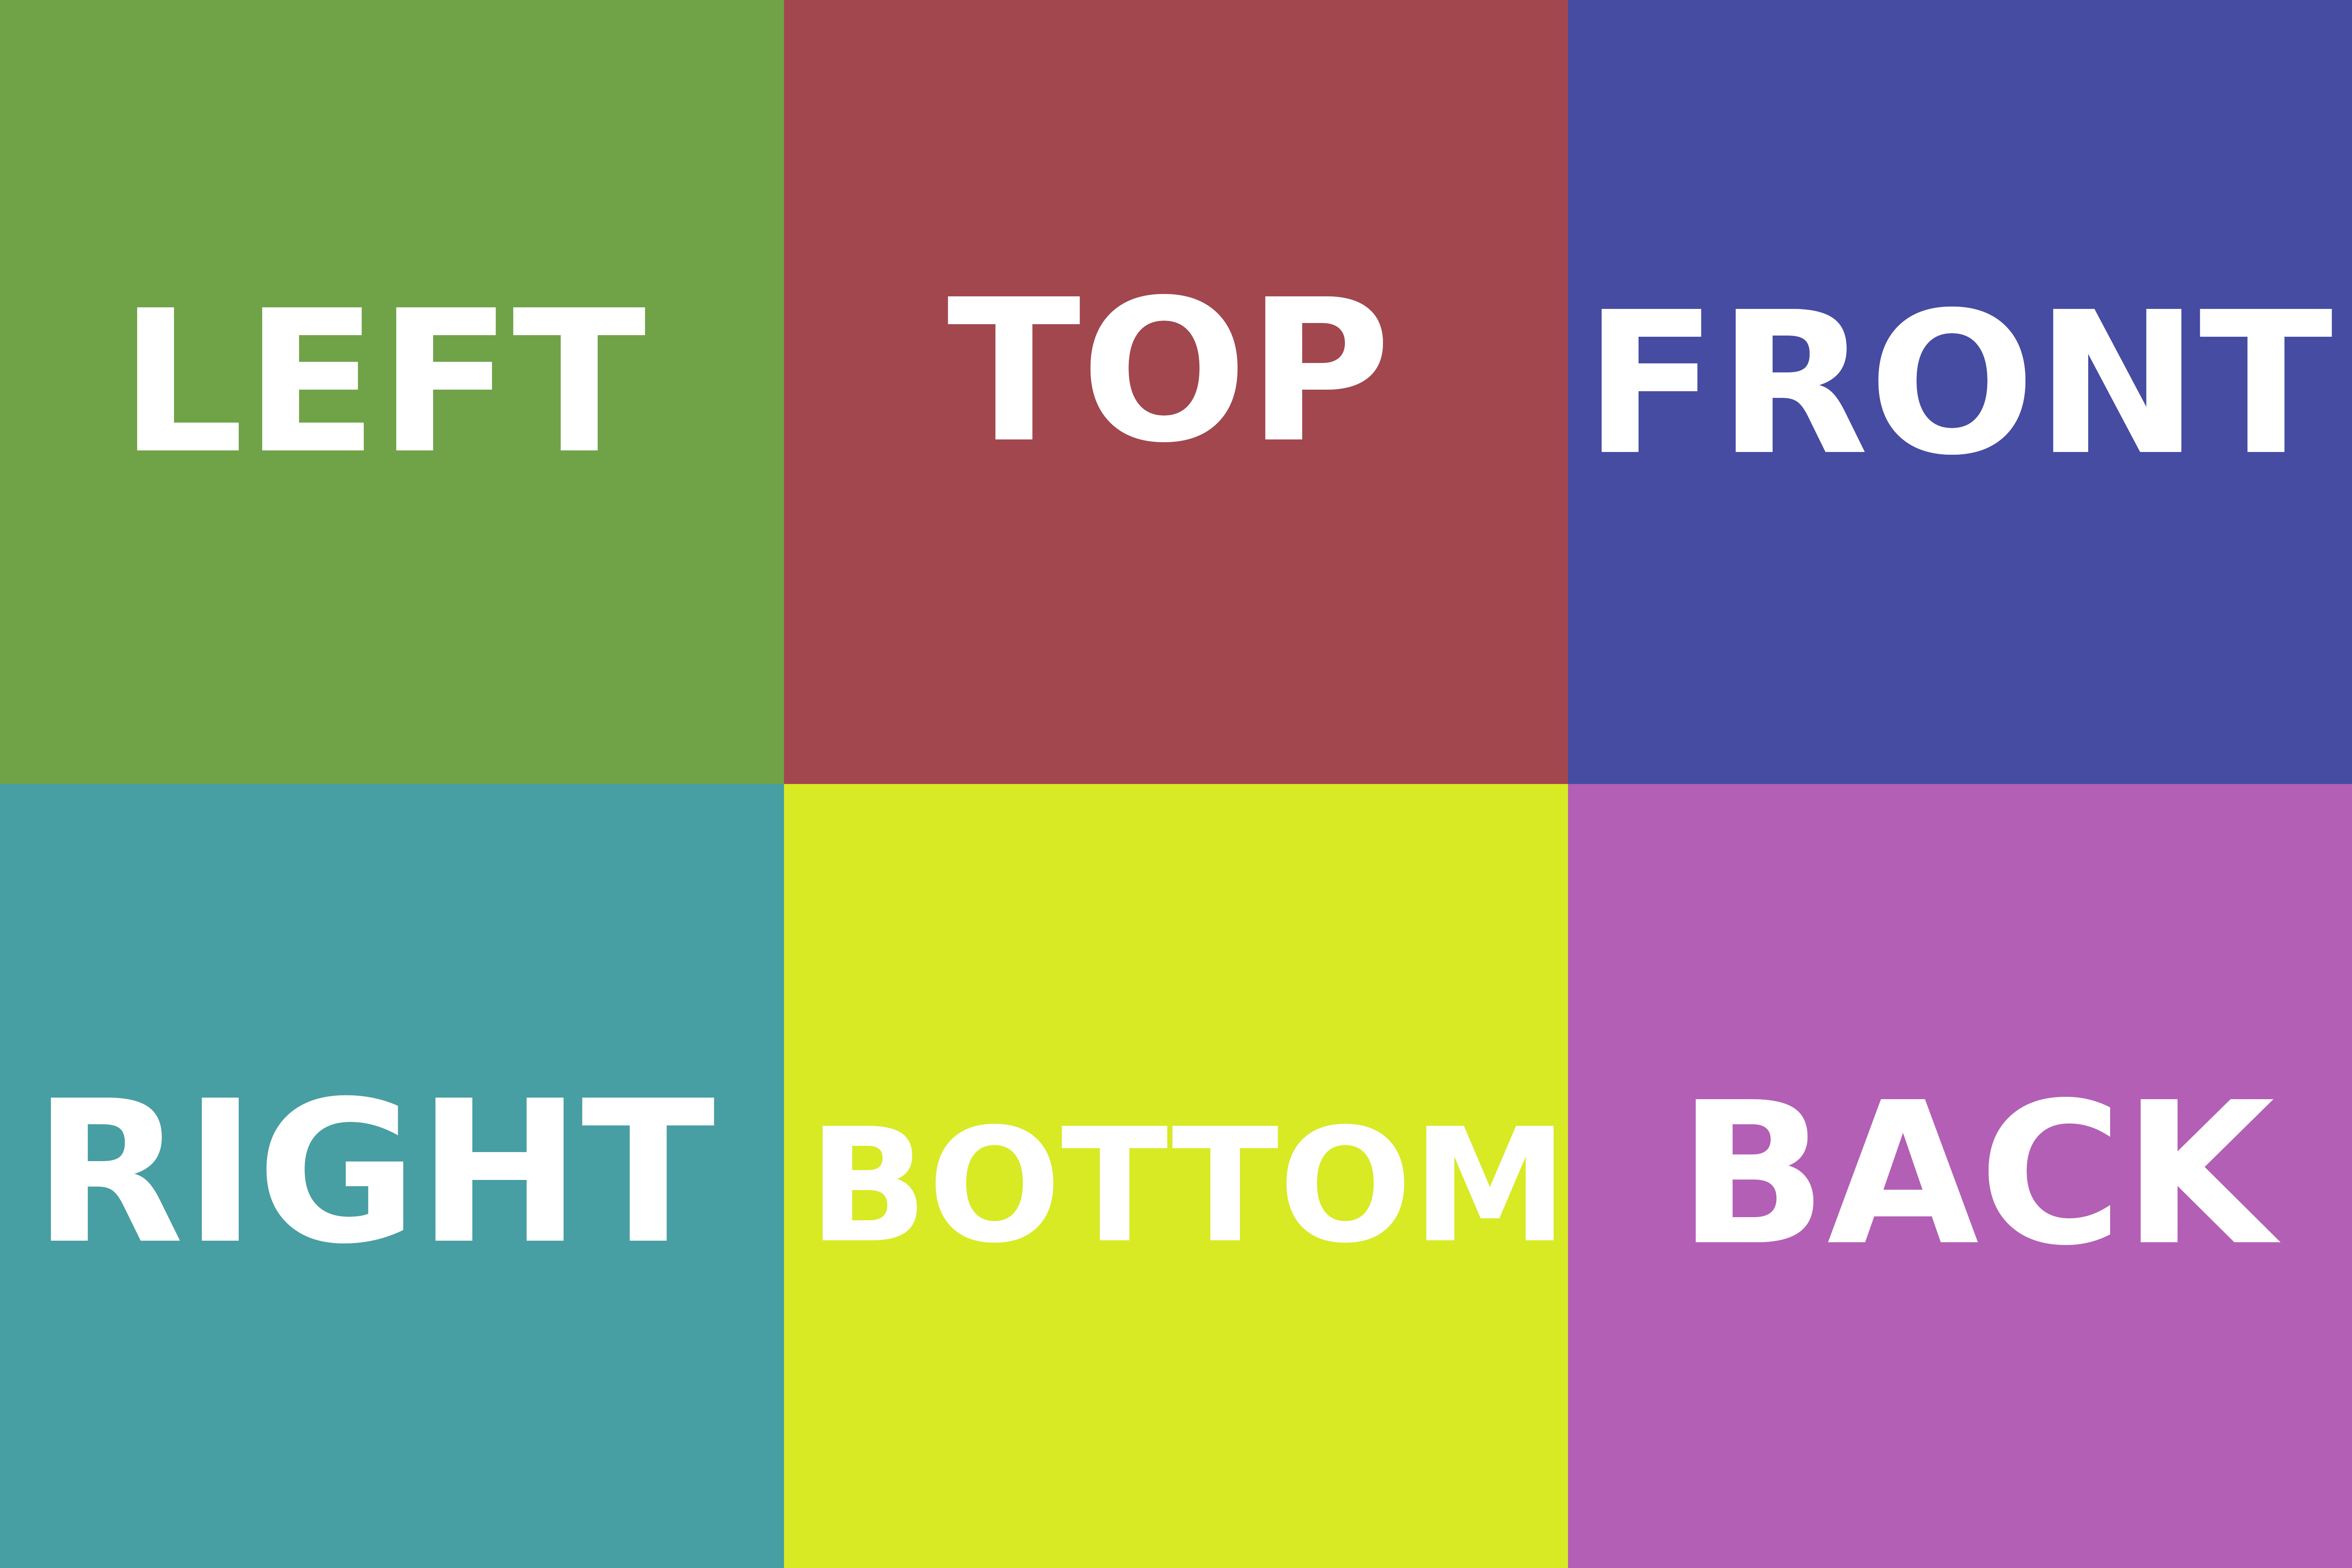
\includegraphics[width=\textwidth]{images/test_cube.jpg}
        \caption{exemplo de textura}
    \end{minipage}\hfill
    \begin{minipage}{0.59\textwidth}
        \centering
        
\includegraphics[width=\textwidth]{images/test_cube_rendered.png}
        \caption{resultado da textura}
    \end{minipage}\hfill
\end{figure}

\section{Patches de Bezier}
Para calcular um \textit{patch de bezier} basta indicar  o nome do ficheiro onde
este se encontra e o nível de \textit{tesselation}.\\
O parsing do ficheiro em questão não foi alterado para esta fase. A única parte
que foi alterada foi a parte de desenhar.\\
Desta forma, convertemos as fórmulas para patches de Bezier de forma a fazer uso
da biblioteca de pontos definida para este trabalho.\\
\begin{figure}[H]
    \centering 
    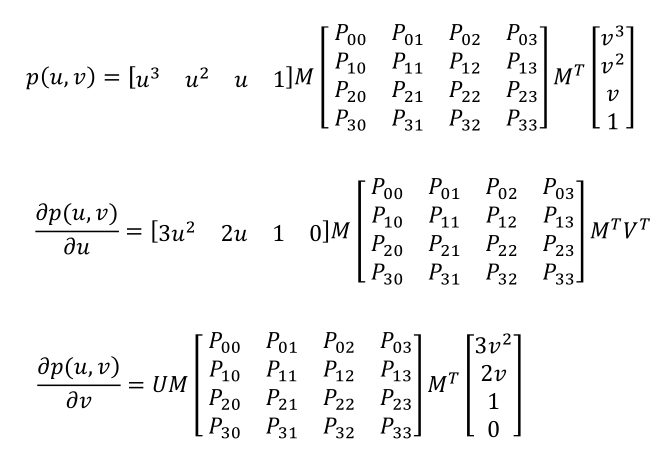
\includegraphics[width=0.4\textwidth]{images/formulas_patches.png}  
    \caption{fórmulas para patches}
\end{figure}
A primeira cabula diretamente as coordenadas do ponto. As duas seguintes
calculam as tangentes no ponto. Desta forma, para obter a normal no ponto é
ainda preciso calcular o \textit{cross product} entre as duas tangentes e
normalizar o resultado.\\
As coordenadas de textura são mapeadas diretamente com base nas coordenadas do
patch que se está a calcular. Assim, para um ponto (u, v) as coordenadas de
textura são dadas por:
\begin{lstlisting}
float x = u / _tesselation_level;
float y = v / _tesselation_level;
\end{lstlisting}

\begin{figure}[H]
    \centering
    \begin{minipage}{0.40\textwidth}
        \centering
        
\includegraphics[width=\textwidth]{images/flowery_patern.jpg}
        \caption{exemplo de textura}
    \end{minipage}\hfill
    \begin{minipage}{0.59\textwidth}
        \centering
        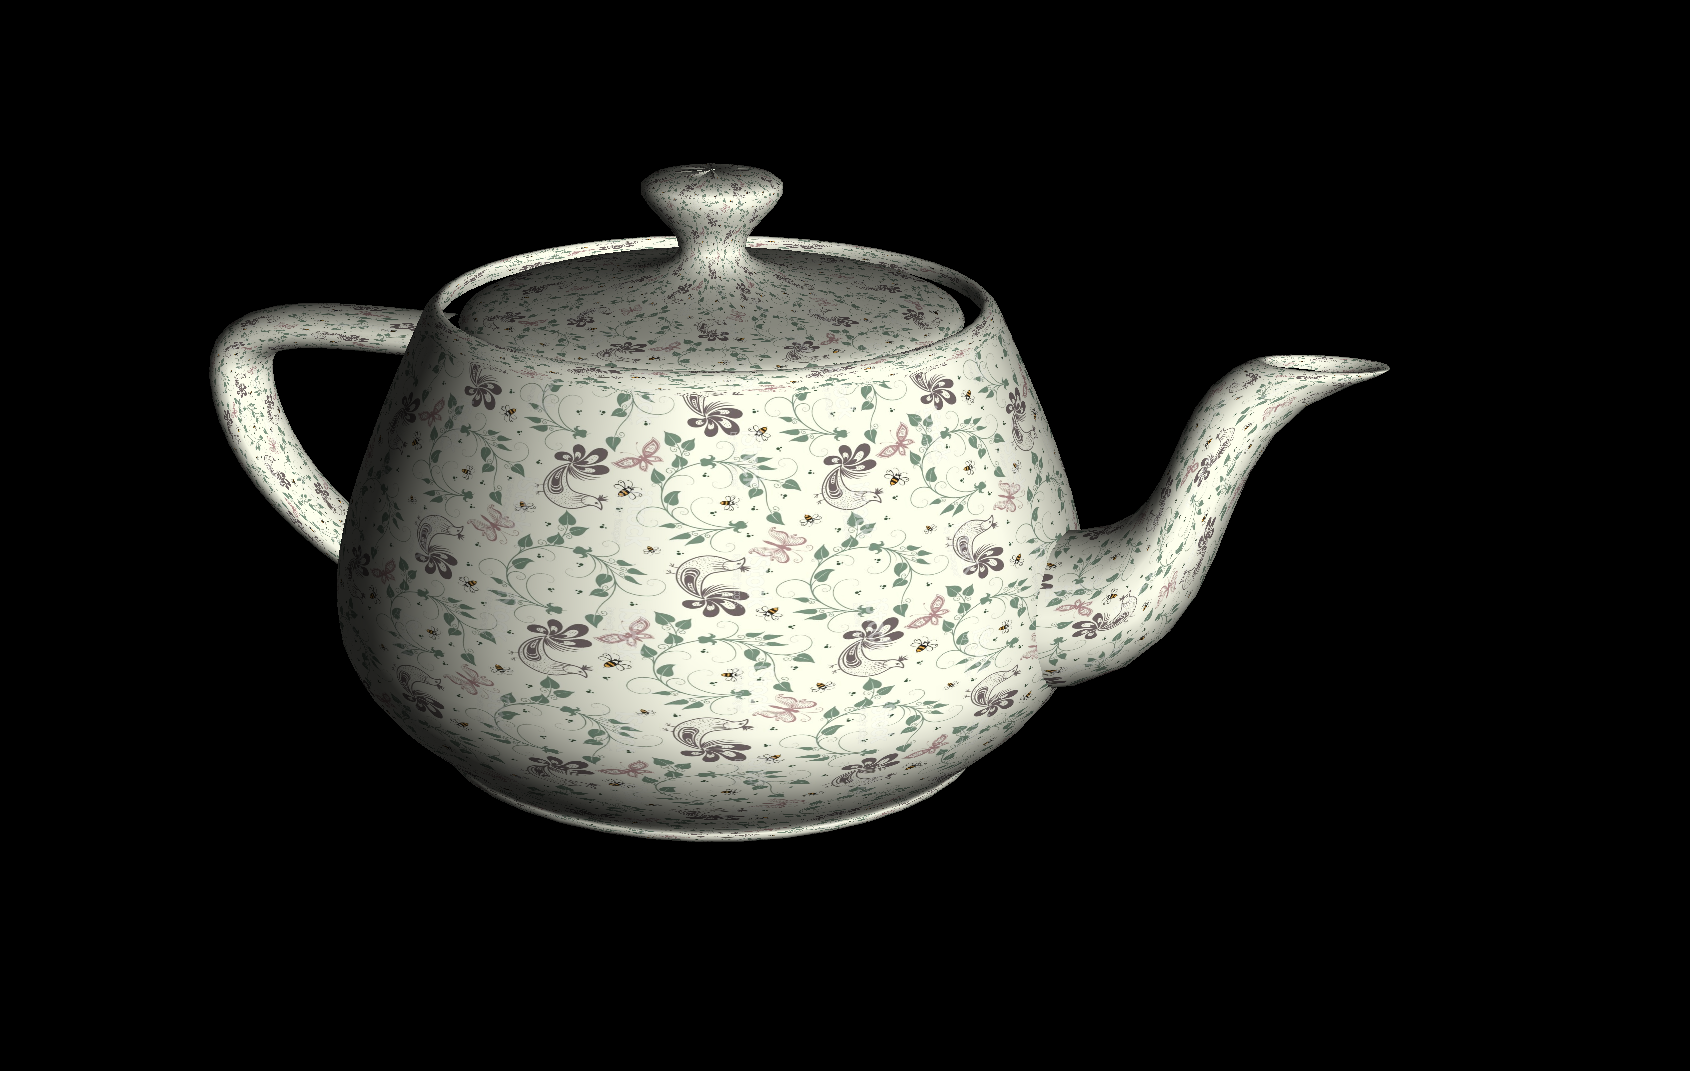
\includegraphics[width=\textwidth]{images/teapot_rendered.png}
        \caption{resultado da textura}
    \end{minipage}\hfill
\end{figure}

\chapter{Engine}
Para facilitar a escrita de scenes mais complexas foram criadas dois extras para
o \textit{engine}. Primeiro é possível passar como argumento múltiplos
ficheiros. Fazendo isto as várias \textit{scenes} serão desenhadas em simultâneo
no ecrã.\\

\section{Buffers}
\subsection{Buffers de Textura}
De forma a guardar a informação de um textura foi criada uma nova classe
chamada \textit{TextureBuffer} que carrega uma textura com base no nome do
ficheiro da textura.\\
Para utilizar esta textura foi criado um método \textit{bind\_texture}.

\subsection{Buffers de Modelos}
De forma análoga, para guardar a informação de um Modelo foi criado uma classe
denominada de \textit{ModelBuffer} que carrega um modelo com base no nome de um
ficheiro .3d definido com o \textit{Generator}. A função \textit{make} devolve
um par com uma instância de \textit{ModelBuffer} e uma \textit{Axis-Aligned
Bounding Box} que engloba o modelo carregado.\\
Para desenhar o modelo foi criado o método \textit{draw\_model} que encapsula
aplicar os 3 buffers no modelo.\\

\subsection{Buffers de Terrenos}
Para guardar a informação de um Terreno foi criada a classe
\textit{TerrainBuffer} que carrega para memória uma imagem e que a converte para
um conjunto de pontos que depois são desenhados por strips. Esta classe, à
semelhança do \textit{ModelBuffer}, contém a função \textit{make} que devolve um
par de \textit{TerrainBuffer} e uma \textit{BoundingBox} com as mesmas
propriedades definidas acima.\\
O código utilizado para computar as normais e as coordenadas de textura é
semelhante ao que foi utilizado na ficha prática número 10 mas modificado para
utilizar o módulo \textit{Point}.\\
Para desenhar o terreno foi criado o método \textit{draw\_terrain} que encapsula
aplicar os 3 buffers no modelo.\\

\subsection{Conjuntos de Buffers}
Visto que pode na mesma \textit{scene} pode ser usado o mesmo modelo, a mesma
textura ou até o mesmo terreno várias vezes não faria sentido estes serem
carregados mais do que uma vez para memória. Desta forma foi criado um buffer
intermédio chamado \textit{GroupBuffer}.\\
Esta classe contém quatro \textit{maps}. O primeiro guarda pares nome de
ficheiro \textit{ModelBuffer}, o segundo guarda pares nome de ficheiro
\textit{TerrainBuffer}, o terceiro guarda pares nome de ficheiro
\textit{TextureBuffer} e o último guarda pares nome de ficheiro
\textit{BoundingBox}.\\
Assim, se se quiser adicionar um Modelo é chamado o método
\textit{insert\_model}. Primeiro verificamos se o Modelo em questão já foi
adicionado. Se ainda não foi adicionado chamamos a função \textit{make} do
\textit{ModelBuffer}, adicionamos o buffer e a \textit{bounding box} aos sítios
respetivos e, por fim, devolvemos a \textit{bounding box}. Se o buffer já tiver
sido adicionado, procurasse no \textit{map} para \textit{bounding boxes} a
respetiva para este modelo e devolve-se.
\begin{lstlisting}
auto search = _model_buffers.find(model_name);
if (search == _model_buffers.end()) {
    auto [model, bb] = ModelBuffer::make(model_name);
    _model_buffers.insert(std::make_pair(model_name, model));
    _bounding_box.insert(std::make_pair(model_name, bb));
    return bb;
} else {
    return _bounding_box[model_name];
}
\end{lstlisting}
O código é igual para os outros dois buffers, com a diferença que no caso de uma
textura nem é inserido nem é devolvido uma \textit{bounding box}.

\section{Objects}
Foi criada uma classe \textit{Object} (com um template para indicar o tipo do
objeto) com o objetivo de guardar informação sobre um dado objeto 3D. Esta
classe contem o nome do ficheiro onde o objeto está guardado, pode conter o nome
do ficheiro da textura caso o objeto tenha textura definida, a cor do objeto, as
cores dos diferentes componentes do material (difuso, especular, emissivo e
ambiente) e a Bounding Box do objeto.\\
Assim, para desenhar um dado objeto basta utilizar o método \textit{draw}.Este
método recebe um \textit{GroupBuffer} e um booleano a indicar se se está a
desenhar em modo de \textit{debug}. Primeiro aplica-se a cor, depois as
propriedades do material, em seguida aplica-se a textura caso exista, depois
desenha-se o modelo com base no valor do template e por fim retira-se a textura.
Caso ainda se esteja em modo de \textit{debug}, desenha-se as \textit{bounding
boxes} do objeto.
\begin{lstlisting}
_colour.apply();

_diffuse.set_diffuse();
_specular.set_specular();
_emissive.set_emissive();
_ambient.set_ambient();

if (_texture_name.has_value()) {
    group_buffer.bind_texture(_texture_name.value());
}

if constexpr (std::is_same_v<T, model_t>) {
    group_buffer.draw_model(_file_name);
} else if constexpr (std::is_same_v<T, terrain_t>) {
    group_buffer.draw_terrain(_file_name);
}

group_buffer.unbind_texture();

if (DEBUG) _bb.draw();
\end{lstlisting}

\section{Parsing de XML}
Para facilitar a construção de um parser e eventual expansão do mesmo foram
criadas pequenas funções que lêem partes mais simples de forma a poder criar um
\textit{Parser Combinator}.\\
Por exemplo, criamos uma função que dado um nodo do \textit{XML}, o nome do
atributo e um valor \textit{default}, verifica se o atributo existe e tem um
valor válido de um float. Caso o valor não seja válido atira um erro com
informação sobre a localização do erro. Caso o atributo não exista devolve o
valor \textit{default}.\\
Este parser é utilizado para a função que lê um ponto três vezes de forma a
conseguir ler as coordenadas do ponto. Seguindo a mesma lógica a função para ler
um vetor utiliza a função de ler um ponto.\\

\subsection{Cor}
Um outro exemplo destes parsers modulares é um parser para ler cor. Este parser
suporta dois formatos distintos: O formato hex que é usado normalmente em design
gráfico (\textit{\#RRGGBBAA} e \textit{\#RRGGBB}) e o formato proposto no
enunciado. Visto que o primeiro é o mais usado nas nossas \textit{scenes} devido
à facilidade de escrita o \textit{parser} dá prioridade de leitura a esse
formato.

\subsection{Include}
Para facilitar ainda mais o processo de separar \textit{scenes} em vários
ficheiros decidimos criar uma extensão do \textit{XML} chamada de
\textit{include}. Com esta tag é possível incluir um ficheiro de \textit{XML}
dentro de outro e quando for desenhado irá herdar as propriedades definidas
anteriormente, nomeadamente a cor.\\
Tal como acontecia previamente, o \textit{GroupBuffer} é partilhado entre os
vários ficheiros. Desta forma mantém-se a premissa que um ficheiro apenas é
carregado uma e uma só vez, independentemente de ser utilizado várias vezes.
Assim, para incluir um ficheiro chamado \textit{lighting.xml} basta colocar a
linha:

\begin{lstlisting}
<include file="lighting.xml">
\end{lstlisting}
Esta extensão foi usada em quase todos os exemplos ao longo deste relatório.
Como o sistema de iluminação é igual para quase todos bastou definir uma scene
onde está definida a iluminação e depois fazer \textit{include} onde foi
necessário utilizar.

\subsection{Object}
Para definir um modelo ou um terreno usa-se a tag model e terrain
respetivamente.\\
Dentro desta tag definem-se o ficheiro a carregar com o atributo \textit{file},
o ficheiro de textura a carregar com o atributo \textit{texture} e as
propriedades definem-se com \textit{diff} para o difuso, \textit{spec} para
specular, \textit{emis} para emissivo e \textit{ambi} para ambiente. Para ler as
propriedades do objeto é usado o parser de cores. Assim, para definir a
propriedade emissiva de um obejto, a linha:
\begin{lstlisting}
emisR="1" emisG="1" emisB="1"
\end{lstlisting}
é equivalente a:
\begin{lstlisting}
emis="#FFFFFF"
\end{lstlisting}


\subsection{Error Handling}
Para facilitar a correção de erros dos ficheiros criamos mensagens de erro que
indicam o ficheiro, a linha e a coluna onde ocorreu o erro. Ainda acrescentamos
uma descrição do erro e, quando relevante, a indicação do atributo.\\
Assim, se ao ler o ficheiro \textit{solar.xml} ocorrer um erro de parsing num
\textit{translate} porque o valor não representa um float o erro terá este
aspeto:
\begin{figure}[H]
    \centering 
    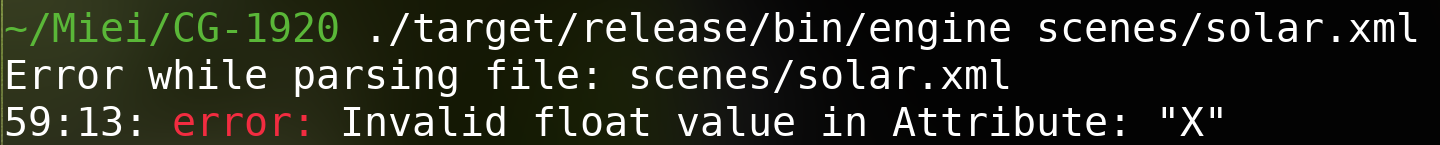
\includegraphics[width=\textwidth]{images/error_handling.png}  
    \caption{Exemplo de erro do praser}
\end{figure}

\chapter{Scenes}
\section{Terrain Generation}
Tal como foi referido acima, a forma como são guardados os buffers garante que
apenas é guardada uma instância de cada ficheiro em memória. \\
Para demonstrar as vantagens deste método criamos um script em python que gera
uma grelha de cubos com altura variável com base numa função de \textit{Perlin
Noise} fazendo com que o terreno final se aproxime bastante do aspeto do jogo
\textit{Minecraft}.\\
O ficheiro gerado em XML encontra-se em \textit{scenes/not\_a\_game.xml}.

\begin{figure}[H]
    \centering 
    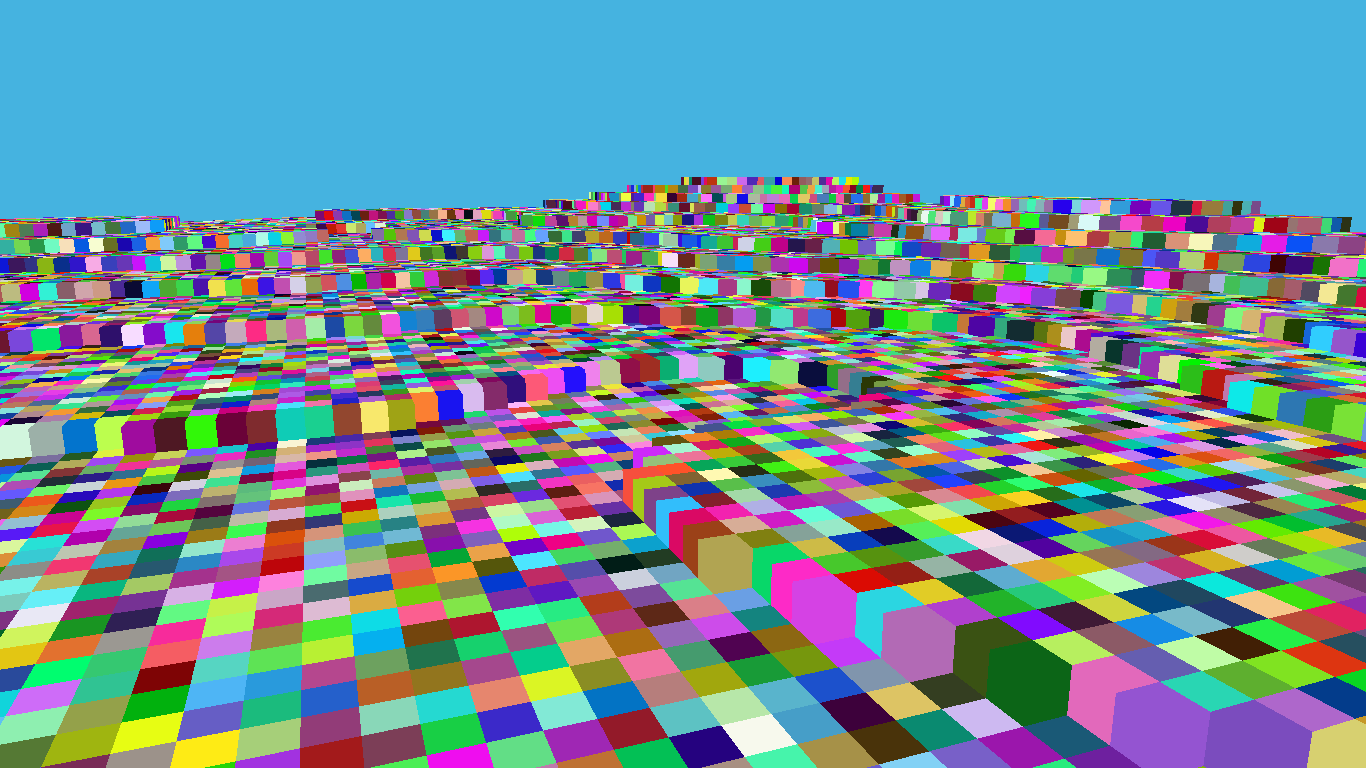
\includegraphics[width=\textwidth]{images/minecraft.png}  
    \caption{Exemplo de terreno gerado}
\end{figure}

\section{Castle in the lake}
Para demonstrar a capacidade das carregar imagens como terreno diretamente no
XML criamos uma \textit{Scene} nova. Nesta desenhamos um castelo numa ilha no
centro de um lago. O Terreno onde se assenta o castelo é desenhado com base num
\textit{HeightMap}.\\
O ficheiro XML encontra-se em \textit{scenes/castle.xml}.

\begin{figure}[H]
    \centering 
    \includegraphics[width=\textwidth]{images/castle.png}  
    \caption{render do \textit{XML} do castelo}
\end{figure}

\section{Solar System}
Para facilitar desenhar o sistema solar decidimos criar um script em Python.\\
Nesta fase melhoramos o script desenvolvido na fase anterior para tirar partido
das alterações feitas ao \textit{engine}.\\
Primeiro adicionamos ao \textit{CSV} obtidos na fase anterior  uma coluna a
indicar qual é a textura de cada planeta.\\
As texturas utilizadas para cada planeta é a que foi possível encontrar com mais
resolução e variam entre 4k e 8k, sendo que a grande maioria está nesta
última.\\
Os anéis de Saturno passaram a ser semi-transparentes e por isso são desenhados
em último lugar.
Adicionamos ainda uma skybox com a textura da via láctea.\\
O ficheiro gerado em XML encontra-se em \textit{scenes/solar.xml}.

\begin{figure}[H]
    \centering 
    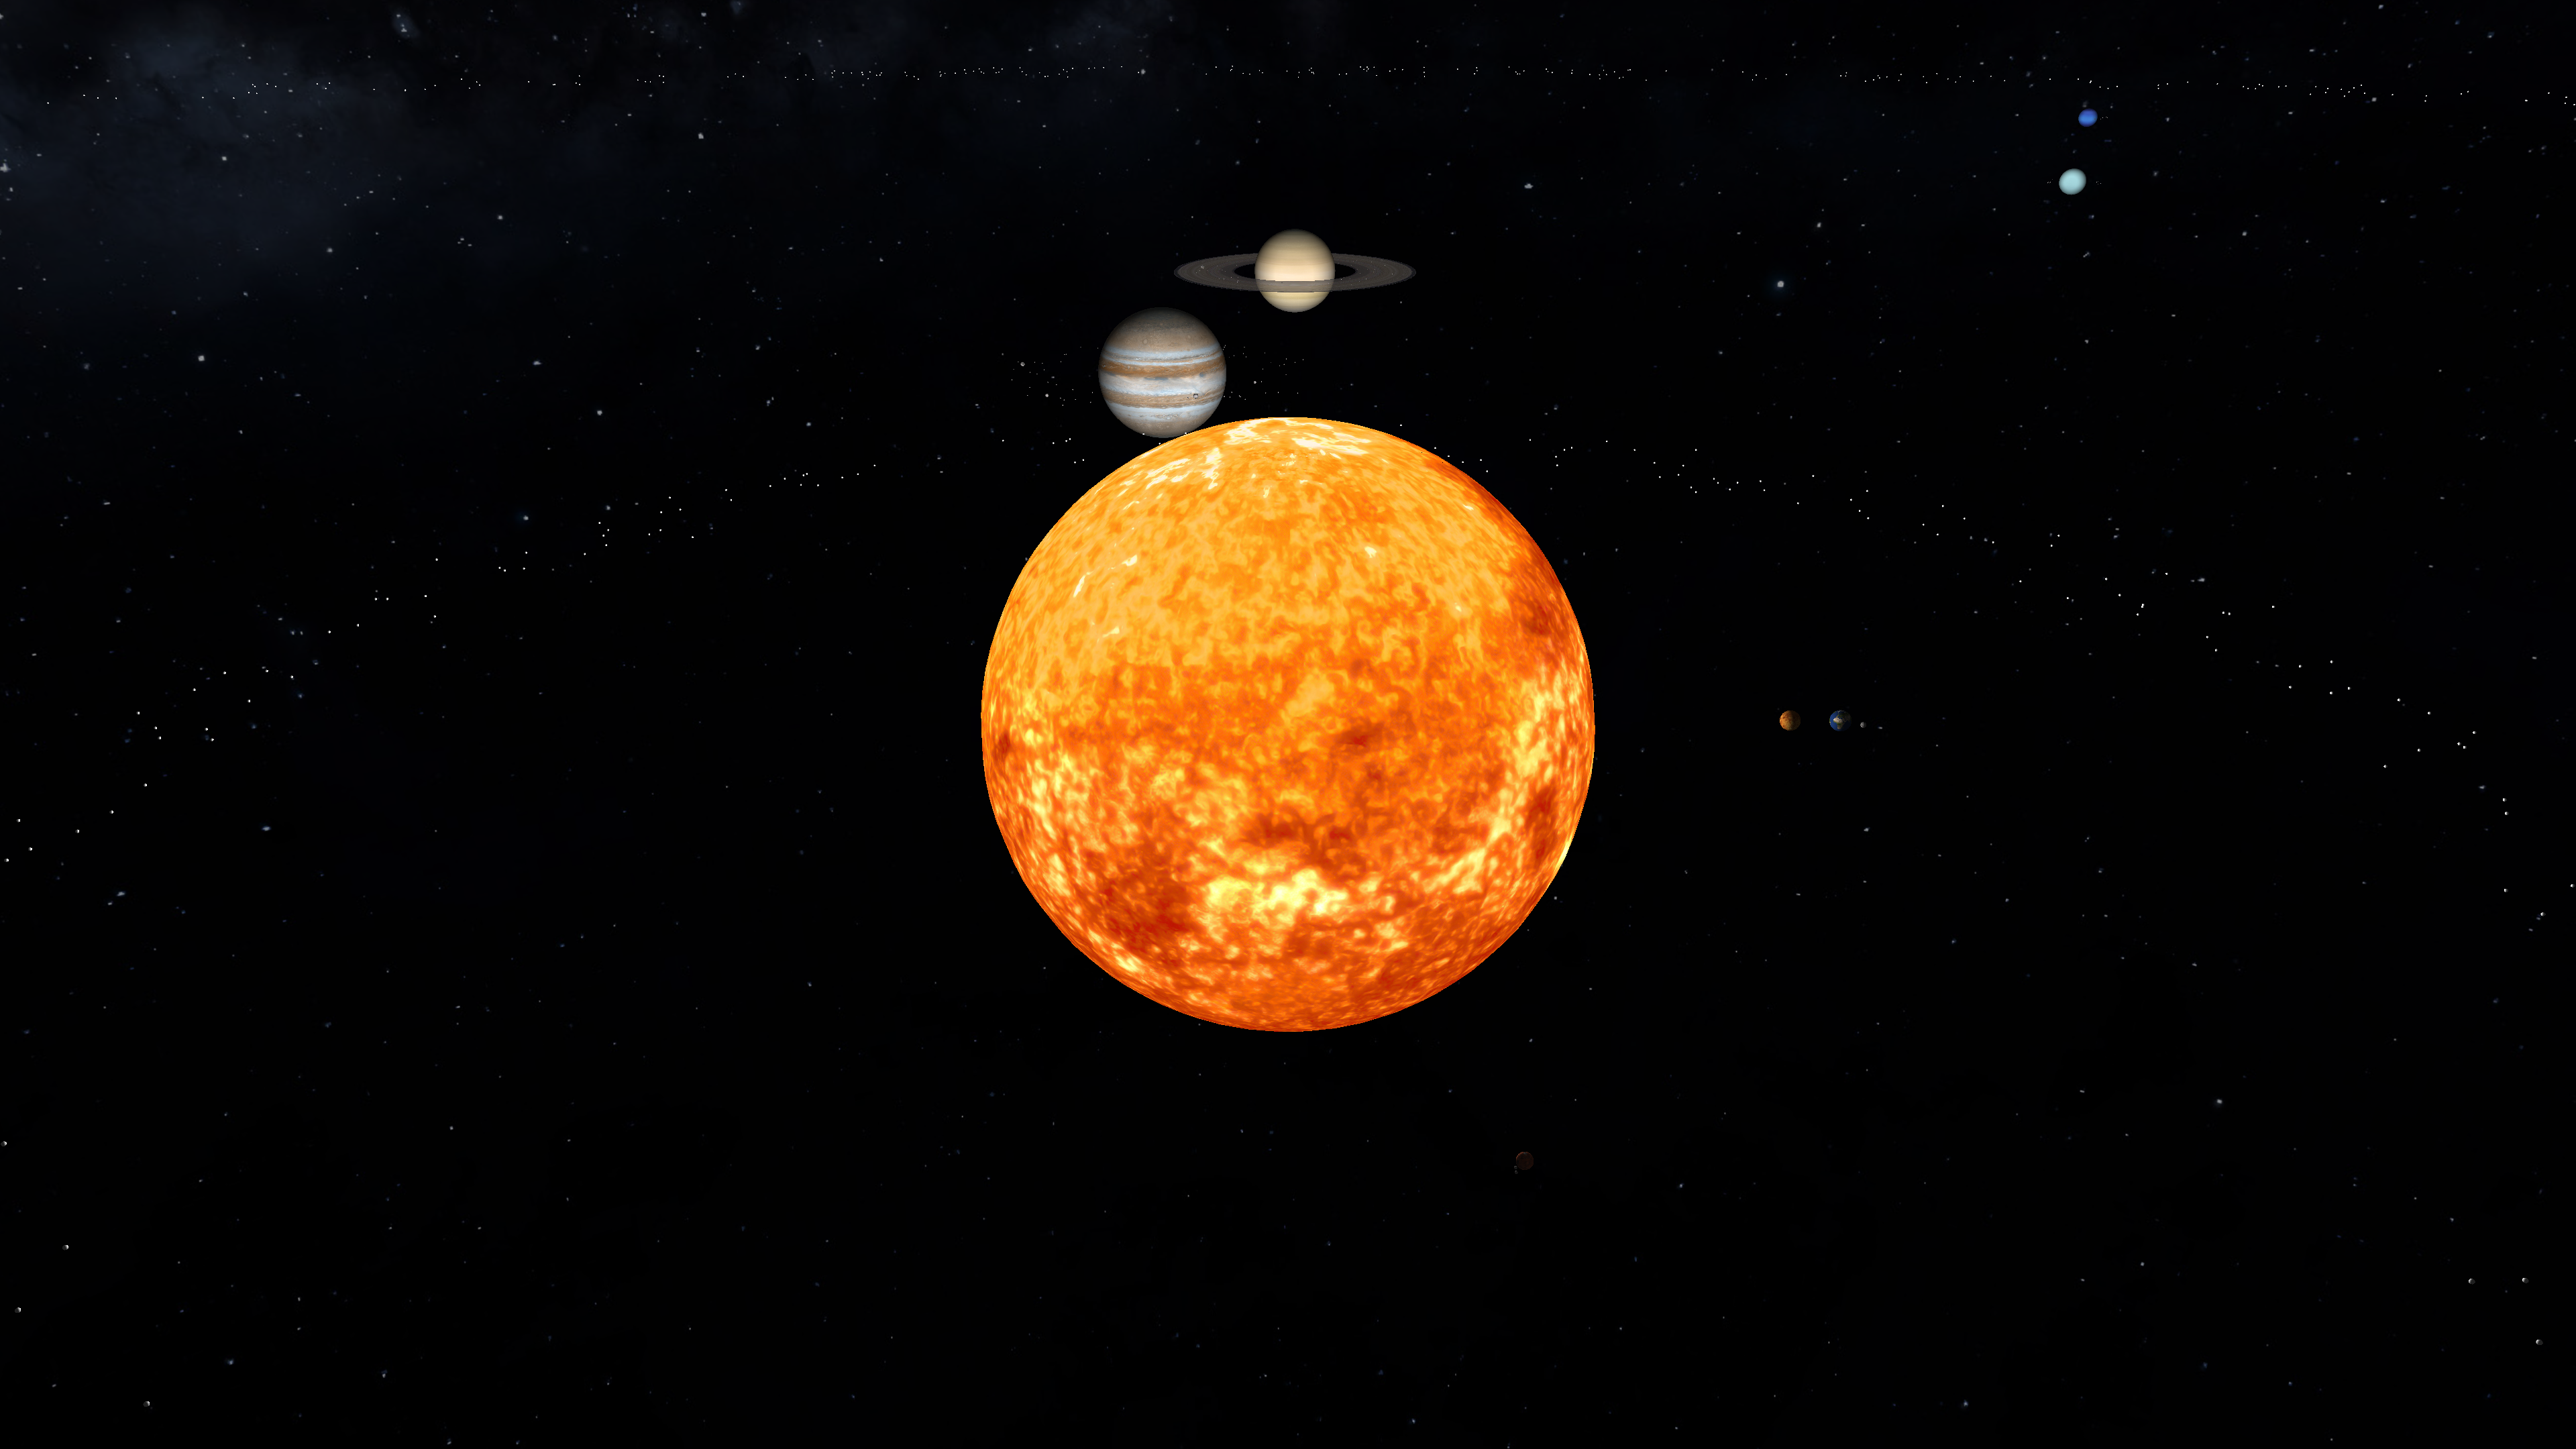
\includegraphics[width=\textwidth]{images/solar_system.png}  
    \caption{Sistema solar}
\end{figure}
\begin{figure}[H]
    \centering 
    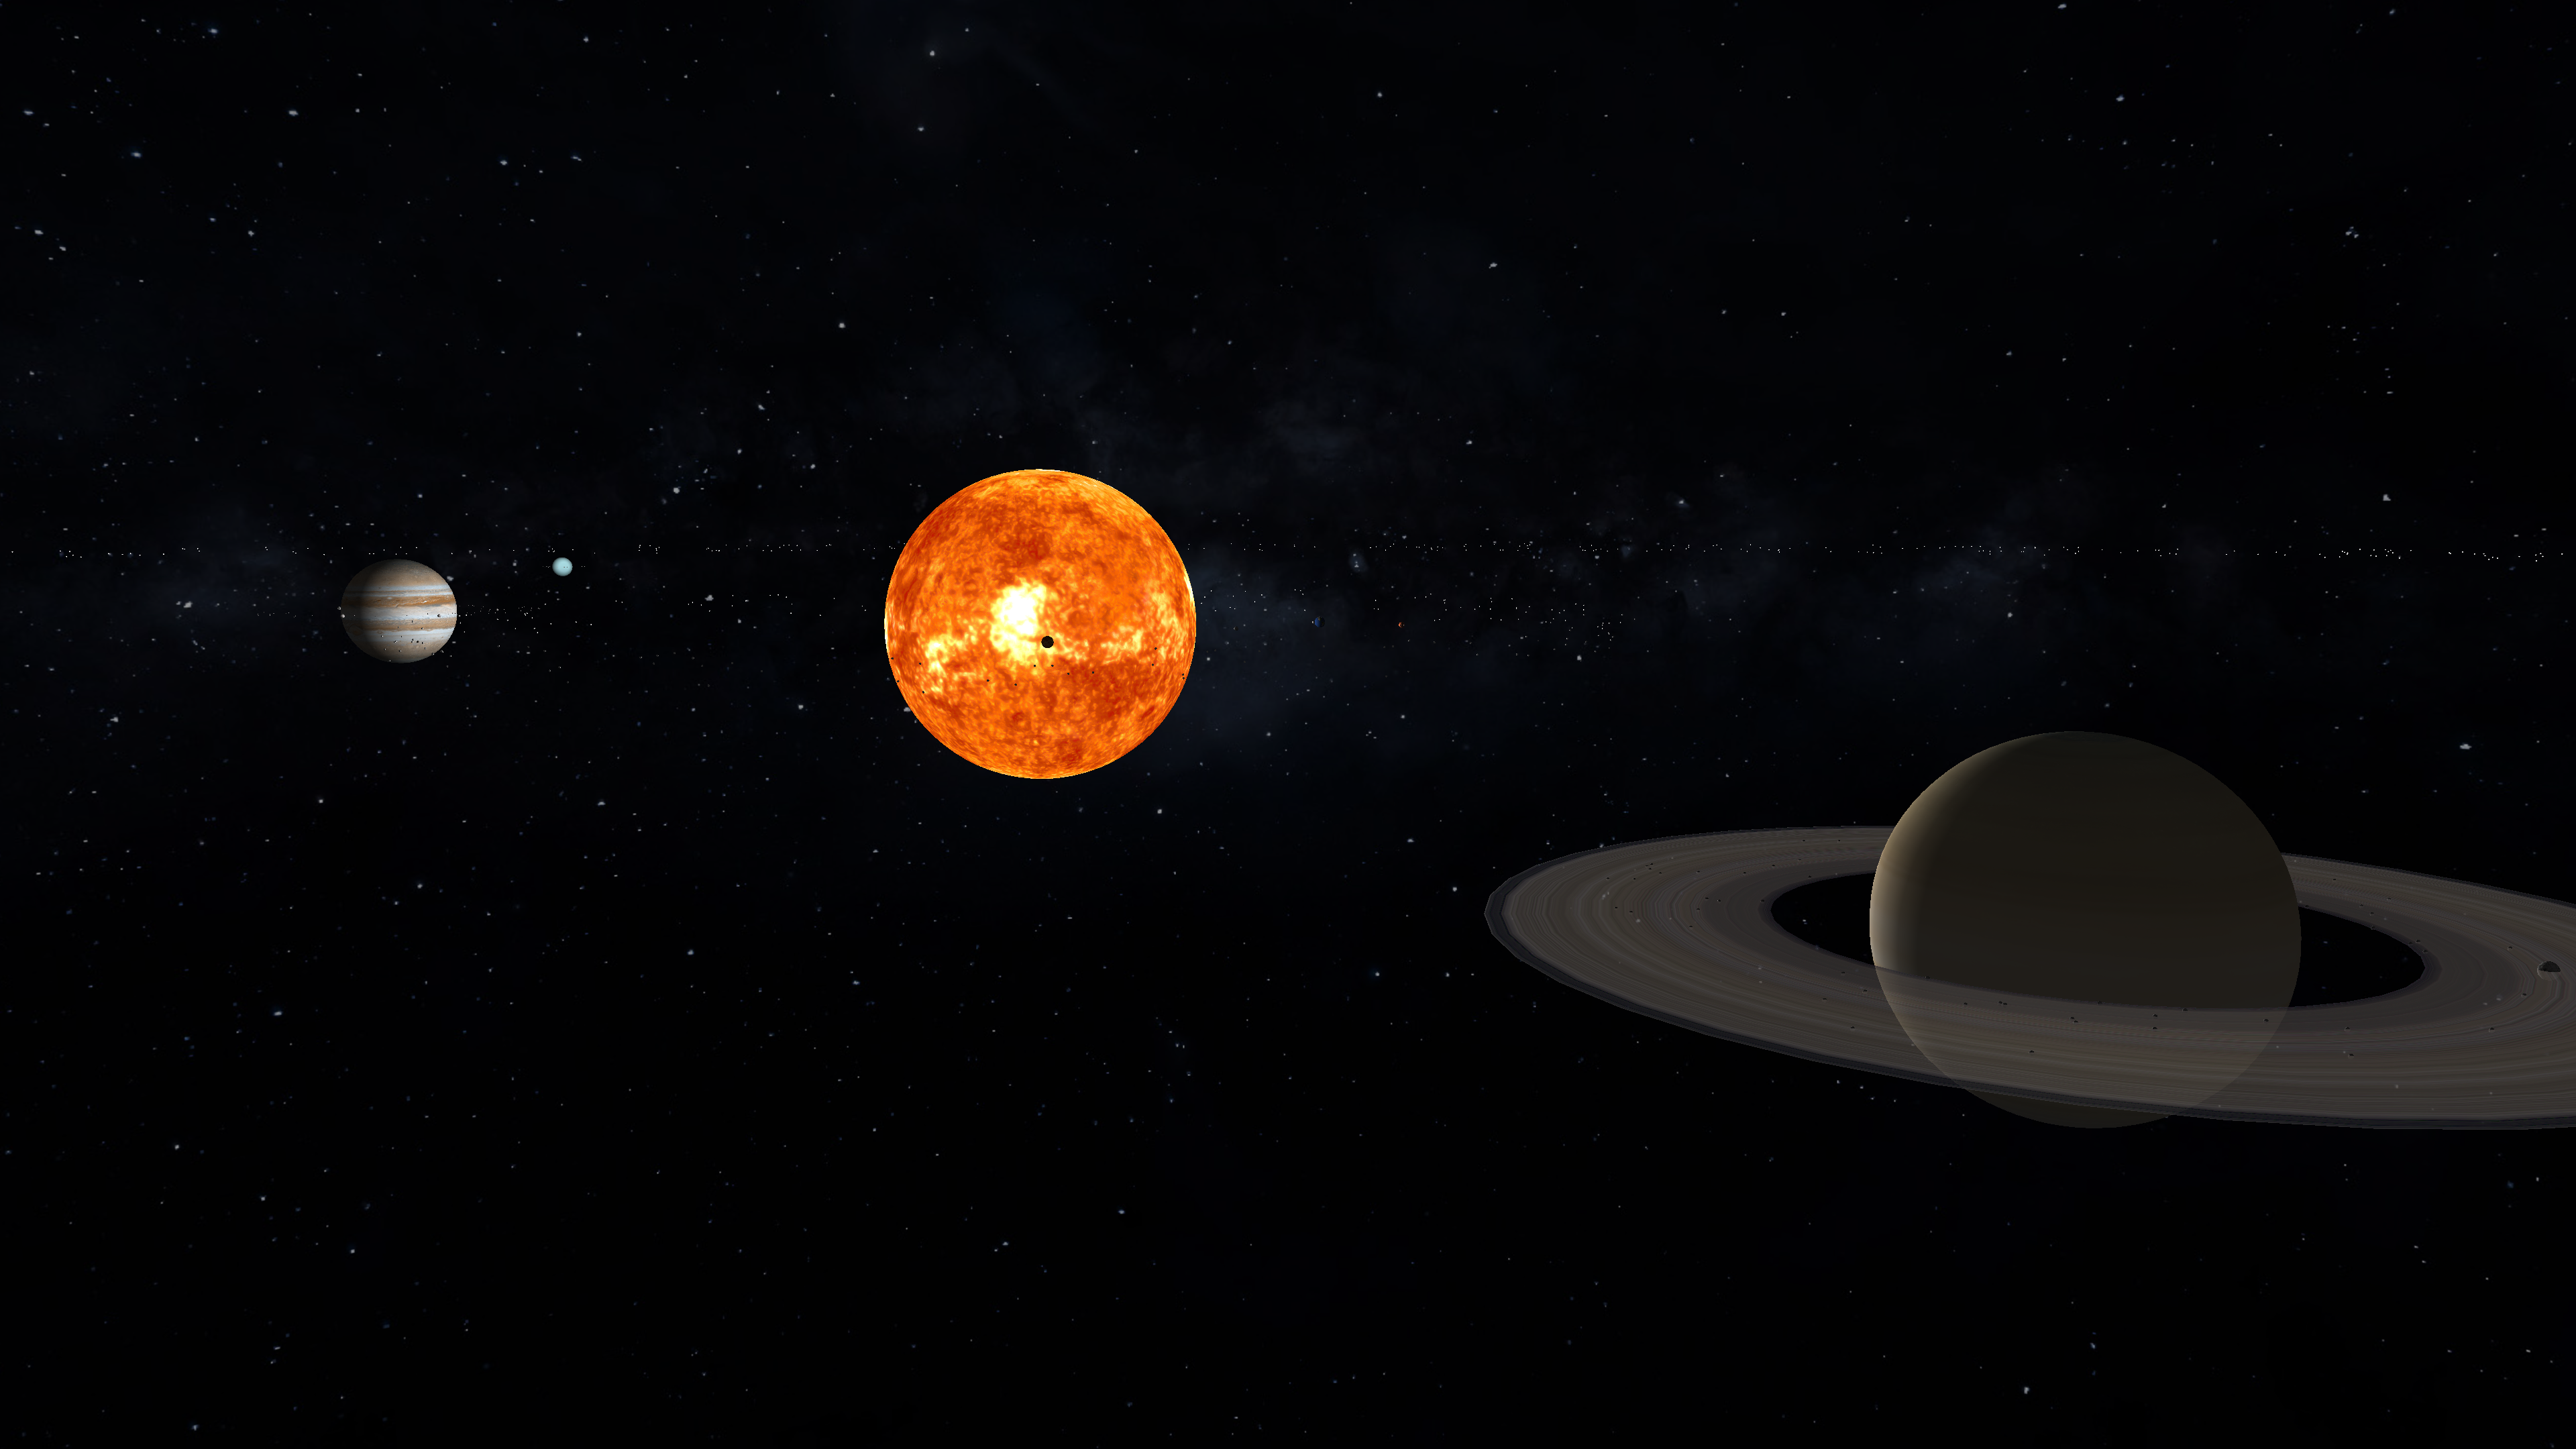
\includegraphics[width=\textwidth]{images/saturn_transparent.png}  
    \caption{Anéis de Saturno transparentes}
\end{figure}
\begin{figure}[H]
    \centering 
    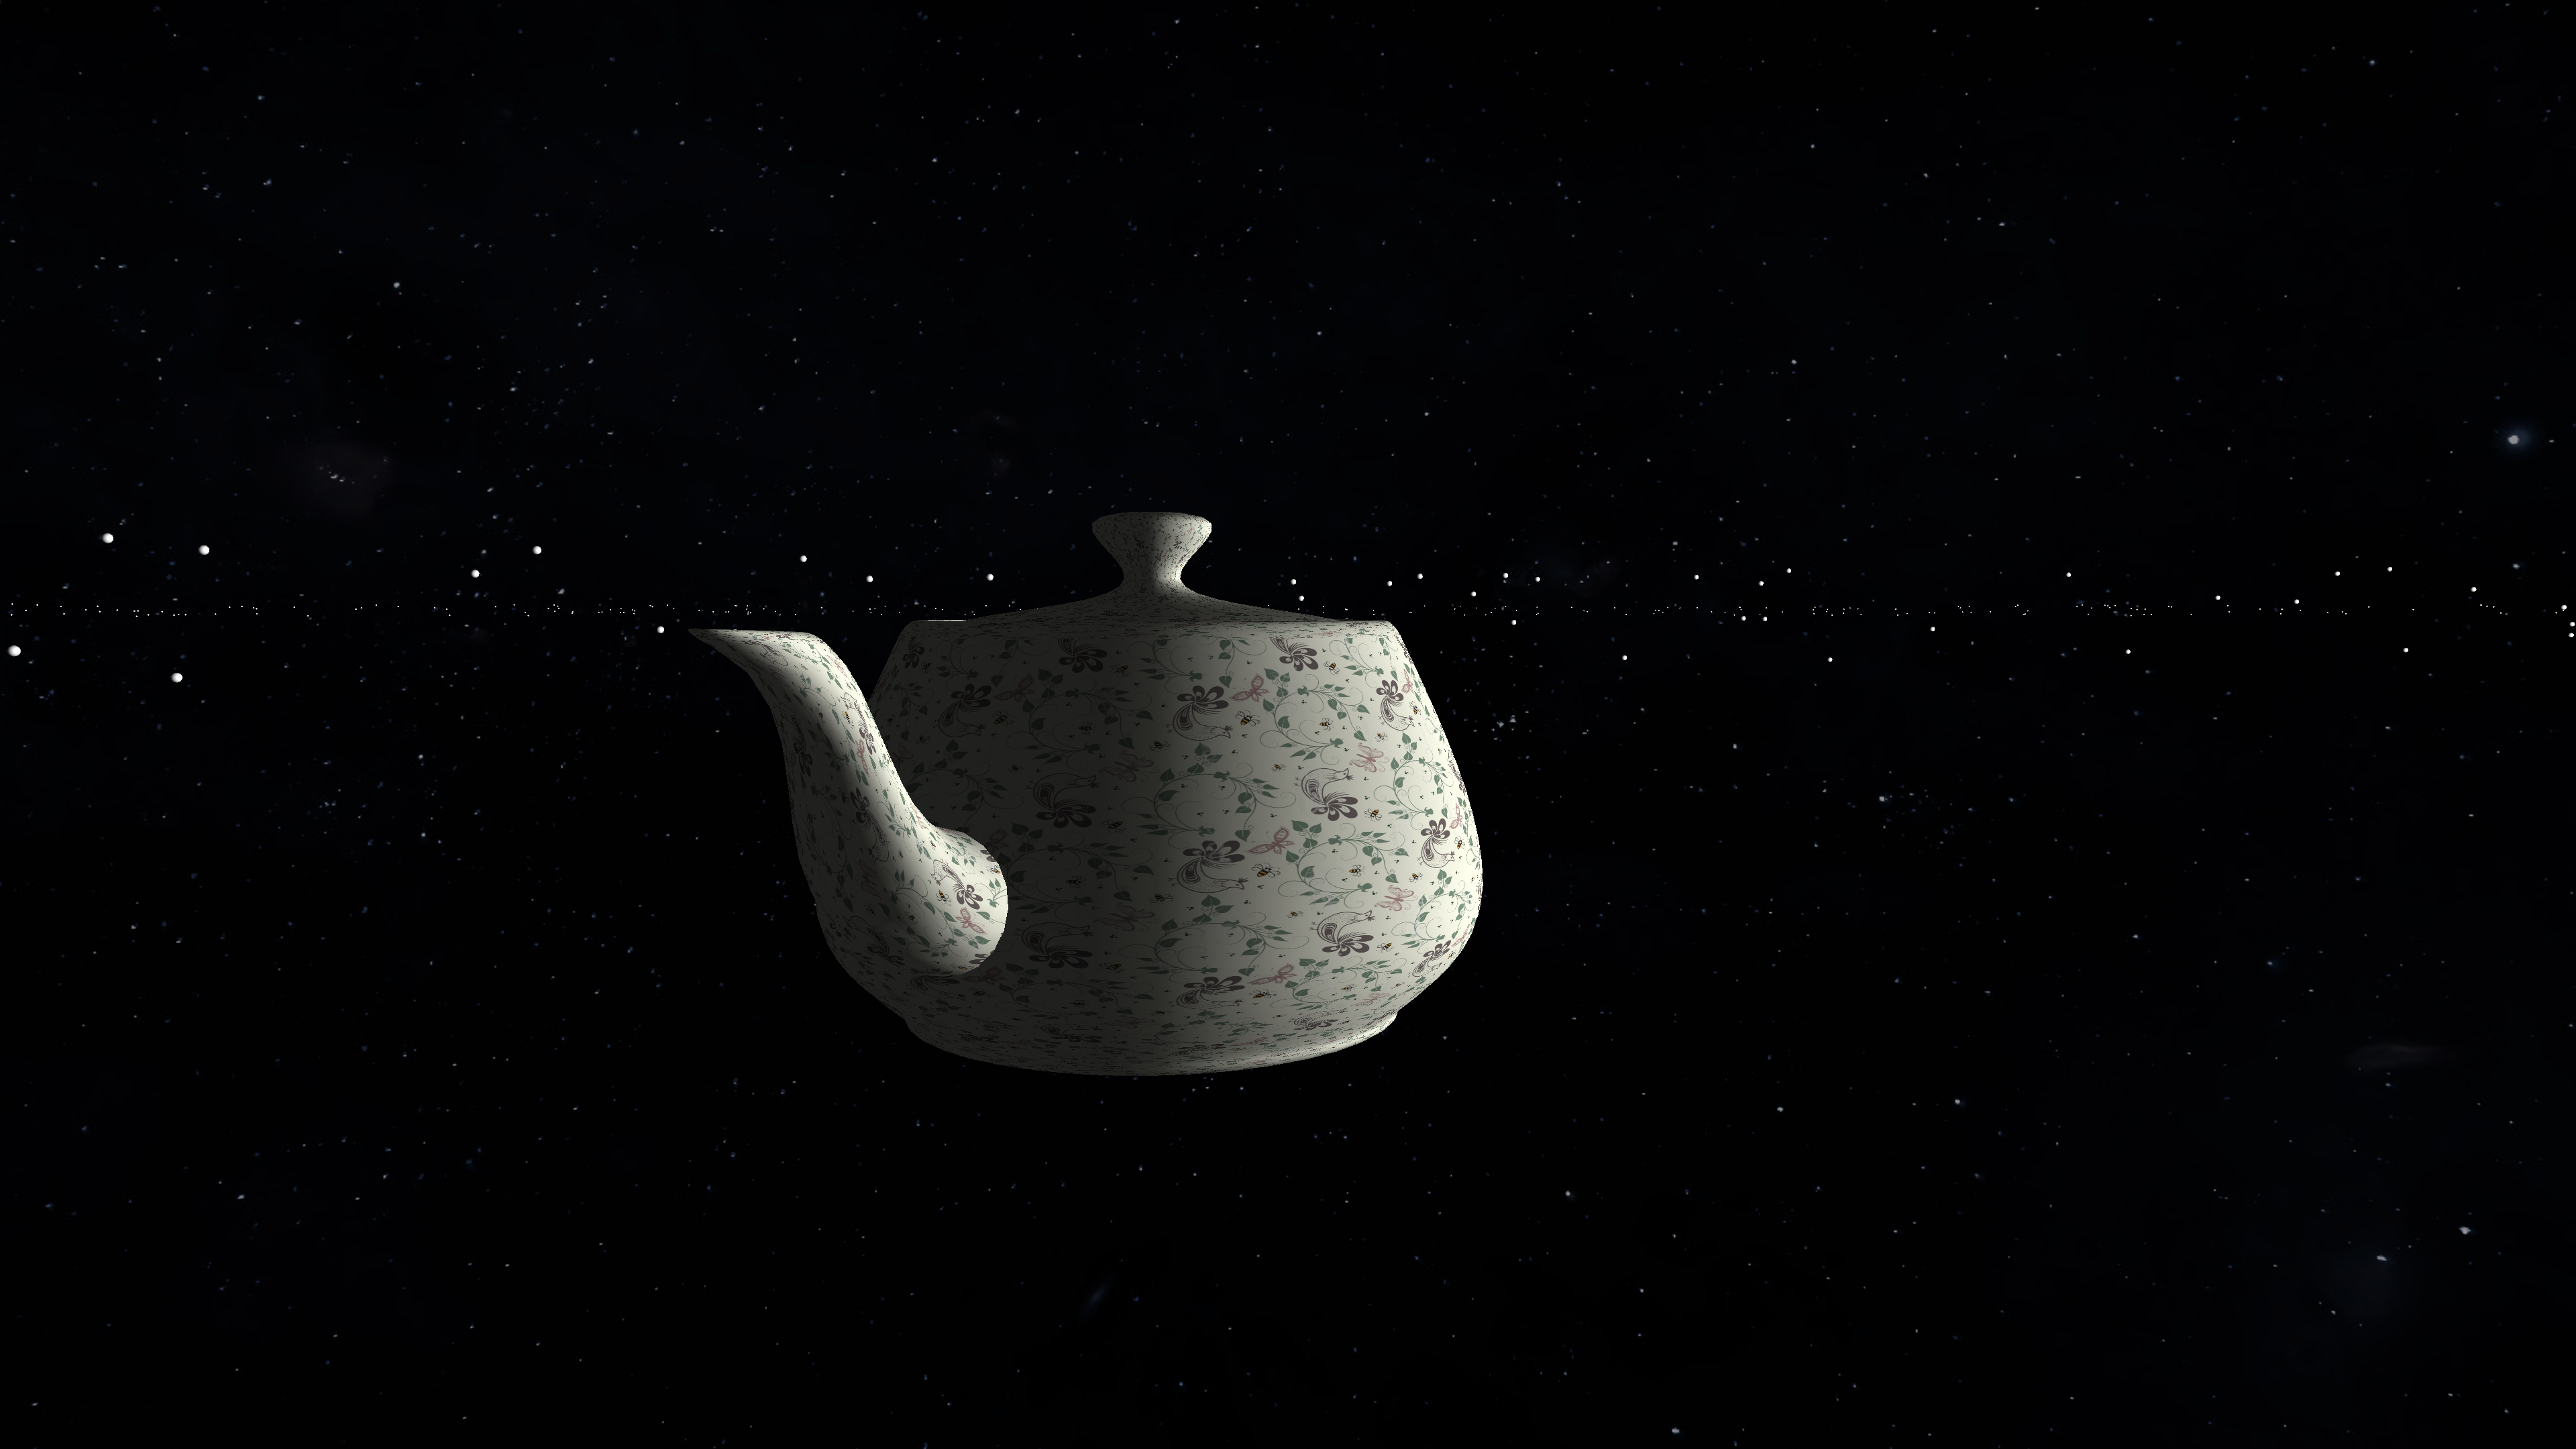
\includegraphics[width=\textwidth]{images/teapot_space.png}  
    \caption{Cometa a usar \textit{patches de bezier}}
\end{figure}
\begin{figure}[H]
    \centering 
    \includegraphics[width=\textwidth]{images/solar_system_debug.png}  
    \caption{Sistema solar em modo de debug com as luzes desligadas}
\end{figure}

\chapter{Conclusão}
Com este trabalho prático podemos aplicar os conhecimentos leccionados até agora
nas aulas da unidade curricular de computação gráfica permitindo assim
aprofundar os nossos conhecimentos de openGl.\\
Como trabalho futuro gostaríamos de acrescentar iluminação e texturas, melhorar
as \textit{scenes} criadas até agora para usarem essas melhorias e acrescentar
mais modos à camera.

\end{document}
